\documentclass[1p]{elsarticle_modified}
%\bibliographystyle{elsarticle-num}

%\usepackage[colorlinks]{hyperref}
%\usepackage{abbrmath_seonhwa} %\Abb, \Ascr, \Acal ,\Abf, \Afrak
\usepackage{amsfonts}
\usepackage{amssymb}
\usepackage{amsmath}
\usepackage{amsthm}
\usepackage{scalefnt}
\usepackage{amsbsy}
\usepackage{kotex}
\usepackage{caption}
\usepackage{subfig}
\usepackage{color}
\usepackage{graphicx}
\usepackage{xcolor} %% white, black, red, green, blue, cyan, magenta, yellow
\usepackage{float}
\usepackage{setspace}
\usepackage{hyperref}

\usepackage{tikz}
\usetikzlibrary{arrows}

\usepackage{multirow}
\usepackage{array} % fixed length table
\usepackage{hhline}

%%%%%%%%%%%%%%%%%%%%%
\makeatletter
\renewcommand*\env@matrix[1][\arraystretch]{%
	\edef\arraystretch{#1}%
	\hskip -\arraycolsep
	\let\@ifnextchar\new@ifnextchar
	\array{*\c@MaxMatrixCols c}}
\makeatother %https://tex.stackexchange.com/questions/14071/how-can-i-increase-the-line-spacing-in-a-matrix
%%%%%%%%%%%%%%%

\usepackage[normalem]{ulem}

\newcommand{\msout}[1]{\ifmmode\text{\sout{\ensuremath{#1}}}\else\sout{#1}\fi}
%SOURCE: \msout is \stkout macro in https://tex.stackexchange.com/questions/20609/strikeout-in-math-mode

\newcommand{\cancel}[1]{
	\ifmmode
	{\color{red}\msout{#1}}
	\else
	{\color{red}\sout{#1}}
	\fi
}

\newcommand{\add}[1]{
	{\color{blue}\uwave{#1}}
}

\newcommand{\replace}[2]{
	\ifmmode
	{\color{red}\msout{#1}}{\color{blue}\uwave{#2}}
	\else
	{\color{red}\sout{#1}}{\color{blue}\uwave{#2}}
	\fi
}

\newcommand{\Sol}{\mathcal{S}} %segment
\newcommand{\D}{D} %diagram
\newcommand{\A}{\mathcal{A}} %arc


%%%%%%%%%%%%%%%%%%%%%%%%%%%%%5 test

\def\sl{\operatorname{\textup{SL}}(2,\Cbb)}
\def\psl{\operatorname{\textup{PSL}}(2,\Cbb)}
\def\quan{\mkern 1mu \triangleright \mkern 1mu}

\theoremstyle{definition}
\newtheorem{thm}{Theorem}[section]
\newtheorem{prop}[thm]{Proposition}
\newtheorem{lem}[thm]{Lemma}
\newtheorem{ques}[thm]{Question}
\newtheorem{cor}[thm]{Corollary}
\newtheorem{defn}[thm]{Definition}
\newtheorem{exam}[thm]{Example}
\newtheorem{rmk}[thm]{Remark}
\newtheorem{alg}[thm]{Algorithm}

\newcommand{\I}{\sqrt{-1}}
\begin{document}

%\begin{frontmatter}
%
%\title{Boundary parabolic representations of knots up to 8 crossings}
%
%%% Group authors per affiliation:
%\author{Yunhi Cho} 
%\address{Department of Mathematics, University of Seoul, Seoul, Korea}
%\ead{yhcho@uos.ac.kr}
%
%
%\author{Seonhwa Kim} %\fnref{s_kim}}
%\address{Center for Geometry and Physics, Institute for Basic Science, Pohang, 37673, Korea}
%\ead{ryeona17@ibs.re.kr}
%
%\author{Hyuk Kim}
%\address{Department of Mathematical Sciences, Seoul National University, Seoul 08826, Korea}
%\ead{hyukkim@snu.ac.kr}
%
%\author{Seokbeom Yoon}
%\address{Department of Mathematical Sciences, Seoul National University, Seoul, 08826,  Korea}
%\ead{sbyoon15@snu.ac.kr}
%
%\begin{abstract}
%We find all boundary parabolic representation of knots up to 8 crossings.
%
%\end{abstract}
%\begin{keyword}
%    \MSC[2010] 57M25 
%\end{keyword}
%
%\end{frontmatter}

%\linenumbers
%\tableofcontents
%
\newcommand\colored[1]{\textcolor{white}{\rule[-0.35ex]{0.8em}{1.4ex}}\kern-0.8em\color{red} #1}%
%\newcommand\colored[1]{\textcolor{white}{ #1}\kern-2.17ex	\textcolor{white}{ #1}\kern-1.81ex	\textcolor{white}{ #1}\kern-2.15ex\color{red}#1	}

{\Large $\underline{12a_{0647}~(K12a_{0647})}$}

\setlength{\tabcolsep}{10pt}
\renewcommand{\arraystretch}{1.6}
\vspace{1cm}\begin{tabular}{m{100pt}>{\centering\arraybackslash}m{274pt}}
\multirow{5}{120pt}{
	\centering
	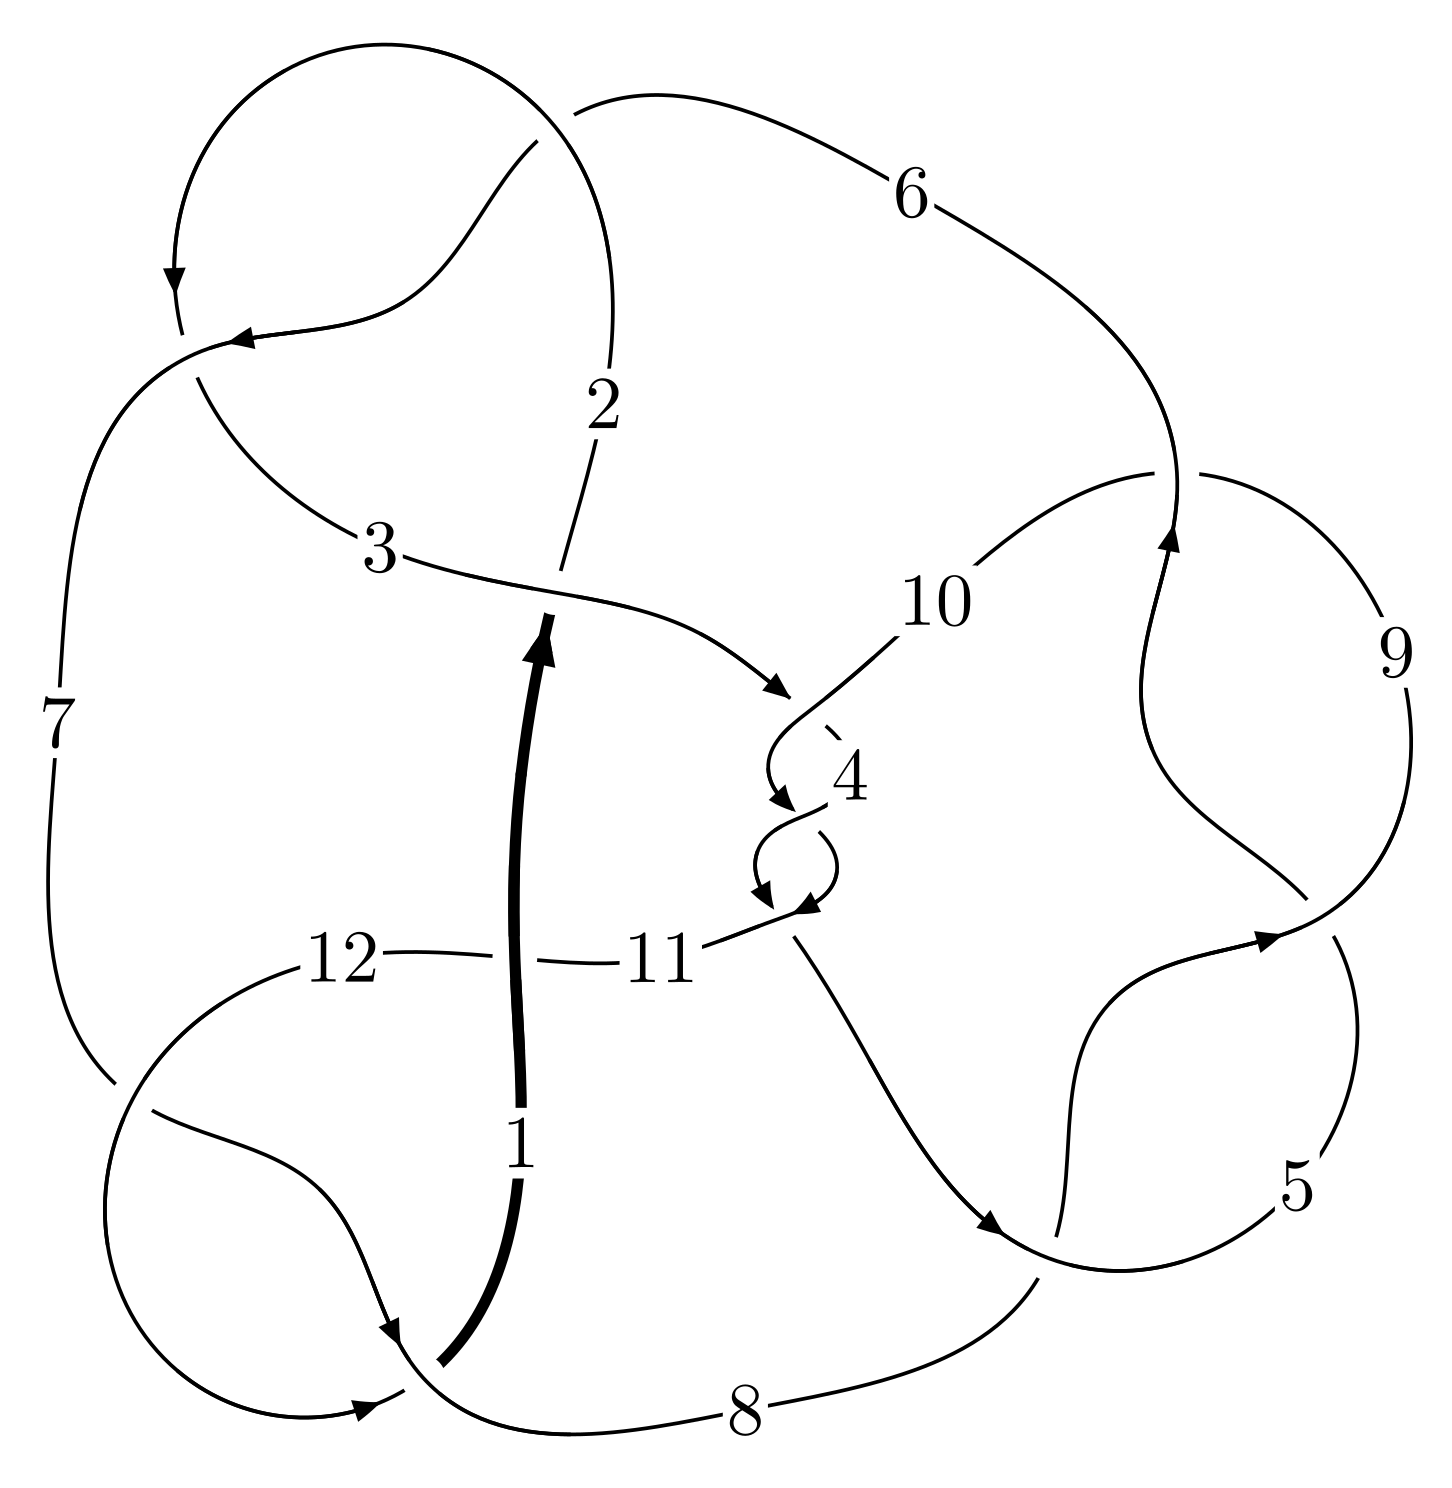
\includegraphics[width=112pt]{../../../GIT/diagram.site/Diagrams/png/1448_12a_0647.png}\\
\ \ \ A knot diagram\footnotemark}&
\allowdisplaybreaks
\textbf{Linearized knot diagam} \\
\cline{2-2}
 &
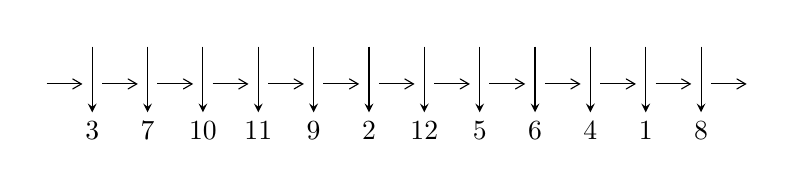
\begin{tikzpicture}[x=20pt, y=17pt]
	% nodes
	\node (C0) at (0, 0) {};
	\node (C1) at (1, 0) {};
	\node (C1U) at (1, +1) {};
	\node (C1D) at (1, -1) {3};

	\node (C2) at (2, 0) {};
	\node (C2U) at (2, +1) {};
	\node (C2D) at (2, -1) {7};

	\node (C3) at (3, 0) {};
	\node (C3U) at (3, +1) {};
	\node (C3D) at (3, -1) {10};

	\node (C4) at (4, 0) {};
	\node (C4U) at (4, +1) {};
	\node (C4D) at (4, -1) {11};

	\node (C5) at (5, 0) {};
	\node (C5U) at (5, +1) {};
	\node (C5D) at (5, -1) {9};

	\node (C6) at (6, 0) {};
	\node (C6U) at (6, +1) {};
	\node (C6D) at (6, -1) {2};

	\node (C7) at (7, 0) {};
	\node (C7U) at (7, +1) {};
	\node (C7D) at (7, -1) {12};

	\node (C8) at (8, 0) {};
	\node (C8U) at (8, +1) {};
	\node (C8D) at (8, -1) {5};

	\node (C9) at (9, 0) {};
	\node (C9U) at (9, +1) {};
	\node (C9D) at (9, -1) {6};

	\node (C10) at (10, 0) {};
	\node (C10U) at (10, +1) {};
	\node (C10D) at (10, -1) {4};

	\node (C11) at (11, 0) {};
	\node (C11U) at (11, +1) {};
	\node (C11D) at (11, -1) {1};

	\node (C12) at (12, 0) {};
	\node (C12U) at (12, +1) {};
	\node (C12D) at (12, -1) {8};
	\node (C13) at (13, 0) {};

	% arrows
	\draw[->,>={angle 60}]
	(C0) edge (C1) (C1) edge (C2) (C2) edge (C3) (C3) edge (C4) (C4) edge (C5) (C5) edge (C6) (C6) edge (C7) (C7) edge (C8) (C8) edge (C9) (C9) edge (C10) (C10) edge (C11) (C11) edge (C12) (C12) edge (C13) ;	\draw[->,>=stealth]
	(C1U) edge (C1D) (C2U) edge (C2D) (C3U) edge (C3D) (C4U) edge (C4D) (C5U) edge (C5D) (C6U) edge (C6D) (C7U) edge (C7D) (C8U) edge (C8D) (C9U) edge (C9D) (C10U) edge (C10D) (C11U) edge (C11D) (C12U) edge (C12D) ;
	\end{tikzpicture} \\
\hhline{~~} \\& 
\textbf{Solving Sequence} \\ \cline{2-2} 
 &
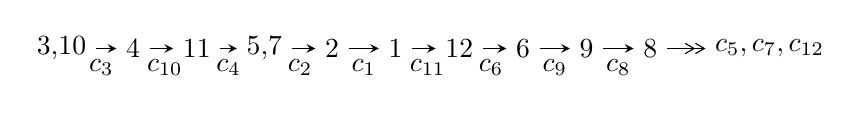
\begin{tikzpicture}[x=23pt, y=7pt]
	% node
	\node (A0) at (-1/8, 0) {3,10};
	\node (A1) at (1, 0) {4};
	\node (A2) at (2, 0) {11};
	\node (A3) at (49/16, 0) {5,7};
	\node (A4) at (33/8, 0) {2};
	\node (A5) at (41/8, 0) {1};
	\node (A6) at (49/8, 0) {12};
	\node (A7) at (57/8, 0) {6};
	\node (A8) at (65/8, 0) {9};
	\node (A9) at (73/8, 0) {8};
	\node (C1) at (1/2, -1) {$c_{3}$};
	\node (C2) at (3/2, -1) {$c_{10}$};
	\node (C3) at (5/2, -1) {$c_{4}$};
	\node (C4) at (29/8, -1) {$c_{2}$};
	\node (C5) at (37/8, -1) {$c_{1}$};
	\node (C6) at (45/8, -1) {$c_{11}$};
	\node (C7) at (53/8, -1) {$c_{6}$};
	\node (C8) at (61/8, -1) {$c_{9}$};
	\node (C9) at (69/8, -1) {$c_{8}$};
	\node (A10) at (11, 0) {$c_{5},c_{7},c_{12}$};

	% edge
	\draw[->,>=stealth]	
	(A0) edge (A1) (A1) edge (A2) (A2) edge (A3) (A3) edge (A4) (A4) edge (A5) (A5) edge (A6) (A6) edge (A7) (A7) edge (A8) (A8) edge (A9) ;
	\draw[->>,>={angle 60}]	
	(A9) edge (A10);
\end{tikzpicture} \\ 

\end{tabular} \\

\footnotetext{
The image of knot diagram is generated by the software ``\textbf{Draw programme}" developed by Andrew Bartholomew(\url{http://www.layer8.co.uk/maths/draw/index.htm\#Running-draw}), where we modified some parts for our purpose(\url{https://github.com/CATsTAILs/LinksPainter}).
}\phantom \\ \newline 
\centering \textbf{Ideals for irreducible components\footnotemark of $X_{\text{par}}$} 
 
\begin{align*}
I^u_{1}&=\langle 
u^{15}-6 u^{14}+\cdots+8 b-10,\;u^{14}-3 u^{13}+\cdots+8 a-2,\;u^{16}-3 u^{15}+\cdots+13 u^2-2\rangle \\
I^u_{2}&=\langle 
9 u^7-7 u^6-24 u^5- u^4+13 u^3+35 u^2+23 b+8 u-39,\\
\phantom{I^u_{2}}&\phantom{= \langle  }66 u^7-13 u^6-153 u^5-107 u^4+149 u^3+249 u^2+161 a-64 u-194,\\
\phantom{I^u_{2}}&\phantom{= \langle  }u^8-2 u^7-2 u^6+4 u^5+3 u^4- u^3-5 u^2-4 u+7\rangle \\
I^u_{3}&=\langle 
- u^{11} a- u^{10} a+\cdots+2 a-3,\;2 u^{11} a- u^{11}+\cdots-4 a+1,\\
\phantom{I^u_{3}}&\phantom{= \langle  }u^{12}+u^{11}-7 u^{10}-6 u^9+18 u^8+11 u^7-19 u^6-2 u^5+6 u^4-8 u^3+1\rangle \\
I^u_{4}&=\langle 
-340 u^{15} a-770 u^{15}+\cdots+249 a+651,\;-180 u^{15} a+621 u^{15}+\cdots-493 a+1534,\\
\phantom{I^u_{4}}&\phantom{= \langle  }u^{16}+u^{15}+\cdots+6 u-1\rangle \\
I^u_{5}&=\langle 
2 a^3+2 a^2+b+5 a+3,\;2 a^4+2 a^3+5 a^2+4 a+1,\;u-1\rangle \\
I^u_{6}&=\langle 
u^3+b- u-1,\;- u^{11}+4 u^9+4 u^8-7 u^7-11 u^6+2 u^5+12 u^4+3 u^3-4 u^2+2 a- u+1,\\
\phantom{I^u_{6}}&\phantom{= \langle  }u^{12}- u^{11}-4 u^{10}+9 u^8+6 u^7-7 u^6-10 u^5-3 u^4+3 u^3+5 u^2+2 u+1\rangle \\
I^u_{7}&=\langle 
b-1,\;6 a+u-3,\;u^2-3\rangle \\
I^u_{8}&=\langle 
-2 a u+4 b+2 a- u+5,\;4 a^2+4 a-7,\;u^2-2 u+1\rangle \\
I^u_{9}&=\langle 
b,\;a+1,\;u+1\rangle \\
I^u_{10}&=\langle 
2 a^3+4 a^2+b+6 a+3,\;2 a^4+4 a^3+6 a^2+4 a+1,\;u+1\rangle \\
\end{align*}\\
\begin{align*}
I^u_{11}&=\langle 
b+1,\;u-1\rangle \\
\\
I^v_{1}&=\langle 
a,\;b-1,\;v+1\rangle \\
\end{align*}
\raggedright * 11 irreducible components of $\dim_{\mathbb{C}}=0$, with total 108 representations.\\
\raggedright * 1 irreducible components of $\dim_{\mathbb{C}}=1$ \\
\footnotetext{All coefficients of polynomials are rational numbers. But the coefficients are sometimes approximated in decimal forms when there is not enough margin.}
\newpage
\renewcommand{\arraystretch}{1}
\centering \section*{I. $I^u_{1}= \langle u^{15}-6 u^{14}+\cdots+8 b-10,\;u^{14}-3 u^{13}+\cdots+8 a-2,\;u^{16}-3 u^{15}+\cdots+13 u^2-2 \rangle$}
\flushleft \textbf{(i) Arc colorings}\\
\begin{tabular}{m{7pt} m{180pt} m{7pt} m{180pt} }
\flushright $a_{3}=$&$\begin{pmatrix}1\\0\end{pmatrix}$ \\
\flushright $a_{10}=$&$\begin{pmatrix}0\\u\end{pmatrix}$ \\
\flushright $a_{4}=$&$\begin{pmatrix}1\\u^2\end{pmatrix}$ \\
\flushright $a_{11}=$&$\begin{pmatrix}- u\\- u^3+u\end{pmatrix}$ \\
\flushright $a_{5}=$&$\begin{pmatrix}- u^2+1\\- u^4+2 u^2\end{pmatrix}$ \\
\flushright $a_{7}=$&$\begin{pmatrix}-\frac{1}{8} u^{14}+\frac{3}{8} u^{13}+\cdots+\frac{1}{2} u+\frac{1}{4}\\-\frac{1}{8} u^{15}+\frac{3}{4} u^{14}+\cdots-\frac{3}{4} u+\frac{5}{4}\end{pmatrix}$ \\
\flushright $a_{2}=$&$\begin{pmatrix}-\frac{1}{8} u^{14}+\frac{3}{8} u^{13}+\cdots+\frac{1}{2} u+\frac{1}{4}\\\frac{5}{8} u^{15}-\frac{3}{2} u^{14}+\cdots+\frac{7}{4} u-\frac{3}{4}\end{pmatrix}$ \\
\flushright $a_{1}=$&$\begin{pmatrix}\frac{5}{8} u^{15}-\frac{13}{8} u^{14}+\cdots+\frac{9}{4} u-\frac{1}{2}\\\frac{5}{8} u^{15}-\frac{3}{2} u^{14}+\cdots+\frac{7}{4} u-\frac{3}{4}\end{pmatrix}$ \\
\flushright $a_{12}=$&$\begin{pmatrix}\frac{1}{8} u^{14}-\frac{3}{8} u^{13}+\cdots-\frac{1}{2} u-\frac{1}{4}\\-\frac{1}{8} u^{15}+\frac{3}{4} u^{14}+\cdots+\frac{5}{4} u+\frac{1}{4}\end{pmatrix}$ \\
\flushright $a_{6}=$&$\begin{pmatrix}1\\\frac{1}{4} u^{15}-\frac{3}{4} u^{14}+\cdots+3 u^2+\frac{1}{2} u\end{pmatrix}$ \\
\flushright $a_{9}=$&$\begin{pmatrix}u\\\frac{1}{4} u^{14}-\frac{3}{4} u^{13}+\cdots+u+\frac{1}{2}\end{pmatrix}$ \\
\flushright $a_{8}=$&$\begin{pmatrix}- u^3+2 u\\\frac{1}{4} u^{14}-\frac{3}{4} u^{13}+\cdots+u+\frac{1}{2}\end{pmatrix}$\\&\end{tabular}
\flushleft \textbf{(ii) Obstruction class $= -1$}\\~\\
\flushleft \textbf{(iii) Cusp Shapes $= \frac{1}{4} u^{15}+\frac{1}{2} u^{14}-\frac{7}{2} u^{13}-\frac{13}{4} u^{12}+16 u^{11}+\frac{25}{4} u^{10}-26 u^9-\frac{15}{4} u^8-2 u^7+3 u^6+\frac{71}{2} u^5+3 u^4-\frac{43}{4} u^3-\frac{73}{4} u^2-\frac{17}{2} u-\frac{25}{2}$}\\~\\
\newpage\renewcommand{\arraystretch}{1}
\flushleft \textbf{(iv) u-Polynomials at the component}\newline \\
\begin{tabular}{m{50pt}|m{274pt}}
Crossings & \hspace{64pt}u-Polynomials at each crossing \\
\hline $$\begin{aligned}c_{1},c_{11}\end{aligned}$$&$\begin{aligned}
&u^{16}+7 u^{15}+\cdots+44 u+4
\end{aligned}$\\
\hline $$\begin{aligned}c_{2},c_{6},c_{7}\\c_{12}\end{aligned}$$&$\begin{aligned}
&u^{16}-3 u^{15}+\cdots+2 u+2
\end{aligned}$\\
\hline $$\begin{aligned}c_{3},c_{4},c_{5}\\c_{8},c_{9},c_{10}\end{aligned}$$&$\begin{aligned}
&u^{16}+3 u^{15}+\cdots+13 u^2-2
\end{aligned}$\\
\hline
\end{tabular}\\~\\
\newpage\renewcommand{\arraystretch}{1}
\flushleft \textbf{(v) Riley Polynomials at the component}\newline \\
\begin{tabular}{m{50pt}|m{274pt}}
Crossings & \hspace{64pt}Riley Polynomials at each crossing \\
\hline $$\begin{aligned}c_{1},c_{11}\end{aligned}$$&$\begin{aligned}
&y^{16}+9 y^{15}+\cdots-912 y+16
\end{aligned}$\\
\hline $$\begin{aligned}c_{2},c_{6},c_{7}\\c_{12}\end{aligned}$$&$\begin{aligned}
&y^{16}-7 y^{15}+\cdots-44 y+4
\end{aligned}$\\
\hline $$\begin{aligned}c_{3},c_{4},c_{5}\\c_{8},c_{9},c_{10}\end{aligned}$$&$\begin{aligned}
&y^{16}-21 y^{15}+\cdots-52 y+4
\end{aligned}$\\
\hline
\end{tabular}\\~\\
\newpage\flushleft \textbf{(vi) Complex Volumes and Cusp Shapes}
$$\begin{array}{c|c|c}  
\text{Solutions to }I^u_{1}& \I (\text{vol} + \sqrt{-1}CS) & \text{Cusp shape}\\
 \hline 
\begin{aligned}
u &= -0.460675 + 0.652431 I \\
a &= -0.24371 - 1.70252 I \\
b &= -1.082390 + 0.575570 I\end{aligned}
 & -0.65793 + 8.23117 I & -13.0423 - 9.7478 I \\ \hline\begin{aligned}
u &= -0.460675 - 0.652431 I \\
a &= -0.24371 + 1.70252 I \\
b &= -1.082390 - 0.575570 I\end{aligned}
 & -0.65793 - 8.23117 I & -13.0423 + 9.7478 I \\ \hline\begin{aligned}
u &= -0.072765 + 0.670397 I \\
a &= \phantom{-}0.742469 + 1.137170 I \\
b &= -0.597448 - 0.616549 I\end{aligned}
 & \phantom{-}2.40804 - 1.30590 I & -6.45602 + 2.87023 I \\ \hline\begin{aligned}
u &= -0.072765 - 0.670397 I \\
a &= \phantom{-}0.742469 - 1.137170 I \\
b &= -0.597448 + 0.616549 I\end{aligned}
 & \phantom{-}2.40804 + 1.30590 I & -6.45602 - 2.87023 I \\ \hline\begin{aligned}
u &= -1.373820 + 0.091320 I \\
a &= \phantom{-}0.060941 - 1.153540 I \\
b &= -0.954330 + 0.864485 I\end{aligned}
 & -4.84234 + 6.50433 I & -18.6838 - 5.6582 I \\ \hline\begin{aligned}
u &= -1.373820 - 0.091320 I \\
a &= \phantom{-}0.060941 + 1.153540 I \\
b &= -0.954330 - 0.864485 I\end{aligned}
 & -4.84234 - 6.50433 I & -18.6838 + 5.6582 I \\ \hline\begin{aligned}
u &= -0.600707 + 0.156541 I \\
a &= \phantom{-}0.458062 - 0.140381 I \\
b &= \phantom{-}0.995675 + 0.611607 I\end{aligned}
 & -1.05898 - 4.82166 I & -12.56614 + 2.63826 I \\ \hline\begin{aligned}
u &= -0.600707 - 0.156541 I \\
a &= \phantom{-}0.458062 + 0.140381 I \\
b &= \phantom{-}0.995675 - 0.611607 I\end{aligned}
 & -1.05898 + 4.82166 I & -12.56614 - 2.63826 I \\ \hline\begin{aligned}
u &= \phantom{-}1.46308 + 0.25525 I \\
a &= \phantom{-}0.482041 - 0.685495 I \\
b &= -0.313593 + 0.976118 I\end{aligned}
 & -7.57778 - 5.08797 I & -15.4427 + 2.0730 I \\ \hline\begin{aligned}
u &= \phantom{-}1.46308 - 0.25525 I \\
a &= \phantom{-}0.482041 + 0.685495 I \\
b &= -0.313593 - 0.976118 I\end{aligned}
 & -7.57778 + 5.08797 I & -15.4427 - 2.0730 I\\
 \hline 
 \end{array}$$\newpage$$\begin{array}{c|c|c}  
\text{Solutions to }I^u_{1}& \I (\text{vol} + \sqrt{-1}CS) & \text{Cusp shape}\\
 \hline 
\begin{aligned}
u &= \phantom{-}1.54279 + 0.38128 I \\
a &= -0.60505 + 1.42874 I \\
b &= -1.251330 - 0.593482 I\end{aligned}
 & -13.5367 - 16.5917 I & -19.8881 + 8.7336 I \\ \hline\begin{aligned}
u &= \phantom{-}1.54279 - 0.38128 I \\
a &= -0.60505 - 1.42874 I \\
b &= -1.251330 + 0.593482 I\end{aligned}
 & -13.5367 + 16.5917 I & -19.8881 - 8.7336 I \\ \hline\begin{aligned}
u &= \phantom{-}0.312284\phantom{ +0.000000I} \\
a &= \phantom{-}0.735032\phantom{ +0.000000I} \\
b &= \phantom{-}0.360485\phantom{ +0.000000I}\end{aligned}
 & -0.574194\phantom{ +0.000000I} & -17.1260\phantom{ +0.000000I} \\ \hline\begin{aligned}
u &= \phantom{-}1.73739 + 0.15693 I \\
a &= \phantom{-}0.464177 + 0.067848 I \\
b &= \phantom{-}1.109290 - 0.308310 I\end{aligned}
 & -17.5882 + 1.3769 I & -22.4716 - 5.7757 I \\ \hline\begin{aligned}
u &= \phantom{-}1.73739 - 0.15693 I \\
a &= \phantom{-}0.464177 - 0.067848 I \\
b &= \phantom{-}1.109290 + 0.308310 I\end{aligned}
 & -17.5882 - 1.3769 I & -22.4716 + 5.7757 I \\ \hline\begin{aligned}
u &= -1.78286\phantom{ +0.000000I} \\
a &= \phantom{-}0.547112\phantom{ +0.000000I} \\
b &= \phantom{-}0.827780\phantom{ +0.000000I}\end{aligned}
 & -15.7038\phantom{ +0.000000I} & -9.77250\phantom{ +0.000000I}\\
 \hline 
 \end{array}$$\newpage\newpage\renewcommand{\arraystretch}{1}
\centering \section*{II. $I^u_{2}= \langle 9 u^7-7 u^6+\cdots+23 b-39,\;66 u^7-13 u^6+\cdots+161 a-194,\;u^8-2 u^7+\cdots-4 u+7 \rangle$}
\flushleft \textbf{(i) Arc colorings}\\
\begin{tabular}{m{7pt} m{180pt} m{7pt} m{180pt} }
\flushright $a_{3}=$&$\begin{pmatrix}1\\0\end{pmatrix}$ \\
\flushright $a_{10}=$&$\begin{pmatrix}0\\u\end{pmatrix}$ \\
\flushright $a_{4}=$&$\begin{pmatrix}1\\u^2\end{pmatrix}$ \\
\flushright $a_{11}=$&$\begin{pmatrix}- u\\- u^3+u\end{pmatrix}$ \\
\flushright $a_{5}=$&$\begin{pmatrix}- u^2+1\\- u^4+2 u^2\end{pmatrix}$ \\
\flushright $a_{7}=$&$\begin{pmatrix}-0.409938 u^{7}+0.0807453 u^{6}+\cdots+0.397516 u+1.20497\\-0.391304 u^{7}+0.304348 u^{6}+\cdots-0.347826 u+1.69565\end{pmatrix}$ \\
\flushright $a_{2}=$&$\begin{pmatrix}0.732919 u^{7}-0.204969 u^{6}+\cdots-0.316770 u-3.36646\\0.130435 u^{7}-0.434783 u^{6}+\cdots-0.217391 u-1.56522\end{pmatrix}$ \\
\flushright $a_{1}=$&$\begin{pmatrix}0.863354 u^{7}-0.639752 u^{6}+\cdots-0.534161 u-4.93168\\0.130435 u^{7}-0.434783 u^{6}+\cdots-0.217391 u-1.56522\end{pmatrix}$ \\
\flushright $a_{12}=$&$\begin{pmatrix}0.0248447 u^{7}+0.298137 u^{6}+\cdots-0.993789 u+0.987578\\0.521739 u^{7}+0.260870 u^{6}+\cdots+1.13043 u-2.26087\end{pmatrix}$ \\
\flushright $a_{6}=$&$\begin{pmatrix}-0.161491 u^{7}+0.0621118 u^{6}+\cdots-0.540373 u-0.919255\\-0.652174 u^{7}+0.173913 u^{6}+\cdots+0.0869565 u+2.82609\end{pmatrix}$ \\
\flushright $a_{9}=$&$\begin{pmatrix}0.118012 u^{7}+0.416149 u^{6}+\cdots+1.27950 u-0.559006\\0.869565 u^{7}-0.565217 u^{6}+\cdots+1.21739 u-3.43478\end{pmatrix}$ \\
\flushright $a_{8}=$&$\begin{pmatrix}0.987578 u^{7}-0.149068 u^{6}+\cdots+0.496894 u-3.99379\\1.17391 u^{7}-0.913043 u^{6}+\cdots-0.956522 u-7.08696\end{pmatrix}$\\&\end{tabular}
\flushleft \textbf{(ii) Obstruction class $= -1$}\\~\\
\flushleft \textbf{(iii) Cusp Shapes $= \frac{12}{23} u^7+\frac{52}{23} u^6-\frac{32}{23} u^5-\frac{124}{23} u^4-\frac{44}{23} u^3+\frac{108}{23} u^2+\frac{72}{23} u-\frac{374}{23}$}\\~\\
\newpage\renewcommand{\arraystretch}{1}
\flushleft \textbf{(iv) u-Polynomials at the component}\newline \\
\begin{tabular}{m{50pt}|m{274pt}}
Crossings & \hspace{64pt}u-Polynomials at each crossing \\
\hline $$\begin{aligned}c_{1},c_{11}\end{aligned}$$&$\begin{aligned}
&(u^4+3 u^3+5 u^2+3 u+1)^2
\end{aligned}$\\
\hline $$\begin{aligned}c_{2},c_{6},c_{7}\\c_{12}\end{aligned}$$&$\begin{aligned}
&(u^4+u^3- u^2- u+1)^2
\end{aligned}$\\
\hline $$\begin{aligned}c_{3},c_{4},c_{5}\\c_{8},c_{9},c_{10}\end{aligned}$$&$\begin{aligned}
&u^8+2 u^7-2 u^6-4 u^5+3 u^4+u^3-5 u^2+4 u+7
\end{aligned}$\\
\hline
\end{tabular}\\~\\
\newpage\renewcommand{\arraystretch}{1}
\flushleft \textbf{(v) Riley Polynomials at the component}\newline \\
\begin{tabular}{m{50pt}|m{274pt}}
Crossings & \hspace{64pt}Riley Polynomials at each crossing \\
\hline $$\begin{aligned}c_{1},c_{11}\end{aligned}$$&$\begin{aligned}
&(y^4+y^3+9 y^2+y+1)^2
\end{aligned}$\\
\hline $$\begin{aligned}c_{2},c_{6},c_{7}\\c_{12}\end{aligned}$$&$\begin{aligned}
&(y^4-3 y^3+5 y^2-3 y+1)^2
\end{aligned}$\\
\hline $$\begin{aligned}c_{3},c_{4},c_{5}\\c_{8},c_{9},c_{10}\end{aligned}$$&$\begin{aligned}
&y^8-8 y^7+26 y^6-42 y^5+35 y^4-27 y^3+59 y^2-86 y+49
\end{aligned}$\\
\hline
\end{tabular}\\~\\
\newpage\flushleft \textbf{(vi) Complex Volumes and Cusp Shapes}
$$\begin{array}{c|c|c}  
\text{Solutions to }I^u_{2}& \I (\text{vol} + \sqrt{-1}CS) & \text{Cusp shape}\\
 \hline 
\begin{aligned}
u &= -0.443967 + 1.001530 I \\
a &= -0.33695 + 1.52789 I \\
b &= \phantom{-}1.192440 - 0.547877 I\end{aligned}
 & -7.14707 + 11.56320 I & -17.7958 - 8.2615 I \\ \hline\begin{aligned}
u &= -0.443967 - 1.001530 I \\
a &= -0.33695 - 1.52789 I \\
b &= \phantom{-}1.192440 + 0.547877 I\end{aligned}
 & -7.14707 - 11.56320 I & -17.7958 + 8.2615 I \\ \hline\begin{aligned}
u &= \phantom{-}1.160120 + 0.413025 I \\
a &= \phantom{-}0.047679 + 0.419061 I \\
b &= -0.692440 + 0.318148 I\end{aligned}
 & -4.36747 + 1.41376 I & -16.2042 - 4.7974 I \\ \hline\begin{aligned}
u &= \phantom{-}1.160120 - 0.413025 I \\
a &= \phantom{-}0.047679 - 0.419061 I \\
b &= -0.692440 - 0.318148 I\end{aligned}
 & -4.36747 - 1.41376 I & -16.2042 + 4.7974 I \\ \hline\begin{aligned}
u &= -1.230820 + 0.345720 I \\
a &= -0.764039 - 0.865204 I \\
b &= -0.692440 + 0.318148 I\end{aligned}
 & -4.36747 + 1.41376 I & -16.2042 - 4.7974 I \\ \hline\begin{aligned}
u &= -1.230820 - 0.345720 I \\
a &= -0.764039 + 0.865204 I \\
b &= -0.692440 - 0.318148 I\end{aligned}
 & -4.36747 - 1.41376 I & -16.2042 + 4.7974 I \\ \hline\begin{aligned}
u &= \phantom{-}1.51466 + 0.24279 I \\
a &= \phantom{-}0.98189 - 1.11892 I \\
b &= \phantom{-}1.192440 + 0.547877 I\end{aligned}
 & -7.14707 - 11.56320 I & -17.7958 + 8.2615 I \\ \hline\begin{aligned}
u &= \phantom{-}1.51466 - 0.24279 I \\
a &= \phantom{-}0.98189 + 1.11892 I \\
b &= \phantom{-}1.192440 - 0.547877 I\end{aligned}
 & -7.14707 + 11.56320 I & -17.7958 - 8.2615 I\\
 \hline 
 \end{array}$$\newpage\newpage\renewcommand{\arraystretch}{1}
\centering \section*{III. $I^u_{3}= \langle - u^{11} a- u^{10} a+\cdots+2 a-3,\;2 u^{11} a- u^{11}+\cdots-4 a+1,\;u^{12}+u^{11}+\cdots-8 u^3+1 \rangle$}
\flushleft \textbf{(i) Arc colorings}\\
\begin{tabular}{m{7pt} m{180pt} m{7pt} m{180pt} }
\flushright $a_{3}=$&$\begin{pmatrix}1\\0\end{pmatrix}$ \\
\flushright $a_{10}=$&$\begin{pmatrix}0\\u\end{pmatrix}$ \\
\flushright $a_{4}=$&$\begin{pmatrix}1\\u^2\end{pmatrix}$ \\
\flushright $a_{11}=$&$\begin{pmatrix}- u\\- u^3+u\end{pmatrix}$ \\
\flushright $a_{5}=$&$\begin{pmatrix}- u^2+1\\- u^4+2 u^2\end{pmatrix}$ \\
\flushright $a_{7}=$&$\begin{pmatrix}a\\\frac{1}{2} u^{11} a+\frac{1}{2} u^{10} a+\cdots- a+\frac{3}{2}\end{pmatrix}$ \\
\flushright $a_{2}=$&$\begin{pmatrix}a\\- u^{11} a- u^{10} a+\cdots+a-\frac{3}{2}\end{pmatrix}$ \\
\flushright $a_{1}=$&$\begin{pmatrix}- u^{11} a- u^{10} a+\cdots+2 a-\frac{3}{2}\\- u^{11} a- u^{10} a+\cdots+a-\frac{3}{2}\end{pmatrix}$ \\
\flushright $a_{12}=$&$\begin{pmatrix}\frac{1}{2} u^{10} a-\frac{1}{2} u^{10}+\cdots-\frac{3}{2} a+\frac{3}{2}\\1\end{pmatrix}$ \\
\flushright $a_{6}=$&$\begin{pmatrix}1\\-\frac{1}{2} u^{11}-\frac{1}{2} u^{10}+\cdots+3 u^2+\frac{1}{2} u\end{pmatrix}$ \\
\flushright $a_{9}=$&$\begin{pmatrix}u\\-\frac{1}{2} u^{10}-\frac{1}{2} u^9+\cdots+u+\frac{1}{2}\end{pmatrix}$ \\
\flushright $a_{8}=$&$\begin{pmatrix}- u^3+2 u\\-\frac{1}{2} u^{10}-\frac{1}{2} u^9+\cdots+u+\frac{1}{2}\end{pmatrix}$\\&\end{tabular}
\flushleft \textbf{(ii) Obstruction class $= -1$}\\~\\
\flushleft \textbf{(iii) Cusp Shapes $= -2 u^{11}- u^{10}+15 u^9+4 u^8-41 u^7+2 u^6+46 u^5-25 u^4-14 u^3+23 u^2-4 u-13$}\\~\\
\newpage\renewcommand{\arraystretch}{1}
\flushleft \textbf{(iv) u-Polynomials at the component}\newline \\
\begin{tabular}{m{50pt}|m{274pt}}
Crossings & \hspace{64pt}u-Polynomials at each crossing \\
\hline $$\begin{aligned}c_{1},c_{11}\end{aligned}$$&$\begin{aligned}
&u^{24}+13 u^{23}+\cdots+280 u+121
\end{aligned}$\\
\hline $$\begin{aligned}c_{2},c_{6},c_{7}\\c_{12}\end{aligned}$$&$\begin{aligned}
&u^{24}-3 u^{23}+\cdots-40 u+11
\end{aligned}$\\
\hline $$\begin{aligned}c_{3},c_{4},c_{5}\\c_{8},c_{9},c_{10}\end{aligned}$$&$\begin{aligned}
&(u^{12}- u^{11}-7 u^{10}+6 u^9+18 u^8-11 u^7-19 u^6+2 u^5+6 u^4+8 u^3+1)^2
\end{aligned}$\\
\hline
\end{tabular}\\~\\
\newpage\renewcommand{\arraystretch}{1}
\flushleft \textbf{(v) Riley Polynomials at the component}\newline \\
\begin{tabular}{m{50pt}|m{274pt}}
Crossings & \hspace{64pt}Riley Polynomials at each crossing \\
\hline $$\begin{aligned}c_{1},c_{11}\end{aligned}$$&$\begin{aligned}
&y^{24}-5 y^{23}+\cdots+60024 y+14641
\end{aligned}$\\
\hline $$\begin{aligned}c_{2},c_{6},c_{7}\\c_{12}\end{aligned}$$&$\begin{aligned}
&y^{24}-13 y^{23}+\cdots-280 y+121
\end{aligned}$\\
\hline $$\begin{aligned}c_{3},c_{4},c_{5}\\c_{8},c_{9},c_{10}\end{aligned}$$&$\begin{aligned}
&(y^{12}-15 y^{11}+\cdots+12 y^2+1)^{2}
\end{aligned}$\\
\hline
\end{tabular}\\~\\
\newpage\flushleft \textbf{(vi) Complex Volumes and Cusp Shapes}
$$\begin{array}{c|c|c}  
\text{Solutions to }I^u_{3}& \I (\text{vol} + \sqrt{-1}CS) & \text{Cusp shape}\\
 \hline 
\begin{aligned}
u &= \phantom{-}0.298602 + 0.646764 I \\
a &= \phantom{-}0.676873 - 0.802179 I \\
b &= -0.385582 + 0.728163 I\end{aligned}
 & \phantom{-}1.36284 - 3.28049 I & -9.00565 + 5.25300 I \\ \hline\begin{aligned}
u &= \phantom{-}0.298602 + 0.646764 I \\
a &= \phantom{-}0.14585 + 1.81517 I \\
b &= -0.956017 - 0.547380 I\end{aligned}
 & \phantom{-}1.36284 - 3.28049 I & -9.00565 + 5.25300 I \\ \hline\begin{aligned}
u &= \phantom{-}0.298602 - 0.646764 I \\
a &= \phantom{-}0.676873 + 0.802179 I \\
b &= -0.385582 - 0.728163 I\end{aligned}
 & \phantom{-}1.36284 + 3.28049 I & -9.00565 - 5.25300 I \\ \hline\begin{aligned}
u &= \phantom{-}0.298602 - 0.646764 I \\
a &= \phantom{-}0.14585 - 1.81517 I \\
b &= -0.956017 + 0.547380 I\end{aligned}
 & \phantom{-}1.36284 + 3.28049 I & -9.00565 - 5.25300 I \\ \hline\begin{aligned}
u &= \phantom{-}1.37505\phantom{ +0.000000I} \\
a &= \phantom{-}0.230814 + 1.020720 I \\
b &= -0.789240 - 0.932040 I\end{aligned}
 & -4.33833\phantom{ +0.000000I} & -18.1100\phantom{ +0.000000I} \\ \hline\begin{aligned}
u &= \phantom{-}1.37505\phantom{ +0.000000I} \\
a &= \phantom{-}0.230814 - 1.020720 I \\
b &= -0.789240 + 0.932040 I\end{aligned}
 & -4.33833\phantom{ +0.000000I} & -18.1100\phantom{ +0.000000I} \\ \hline\begin{aligned}
u &= \phantom{-}0.527999\phantom{ +0.000000I} \\
a &= \phantom{-}0.534112 + 0.186718 I \\
b &= \phantom{-}0.668373 - 0.583240 I\end{aligned}
 & -0.0415570\phantom{ +0.000000I} & -11.1730\phantom{ +0.000000I} \\ \hline\begin{aligned}
u &= \phantom{-}0.527999\phantom{ +0.000000I} \\
a &= \phantom{-}0.534112 - 0.186718 I \\
b &= \phantom{-}0.668373 + 0.583240 I\end{aligned}
 & -0.0415570\phantom{ +0.000000I} & -11.1730\phantom{ +0.000000I} \\ \hline\begin{aligned}
u &= -1.50349 + 0.33368 I \\
a &= \phantom{-}0.486081 + 0.616876 I \\
b &= -0.211945 - 1.000110 I\end{aligned}
 & -10.3396 + 10.8681 I & -17.3574 - 5.7403 I \\ \hline\begin{aligned}
u &= -1.50349 + 0.33368 I \\
a &= -0.48833 - 1.44566 I \\
b &= -1.209730 + 0.620883 I\end{aligned}
 & -10.3396 + 10.8681 I & -17.3574 - 5.7403 I\\
 \hline 
 \end{array}$$\newpage$$\begin{array}{c|c|c}  
\text{Solutions to }I^u_{3}& \I (\text{vol} + \sqrt{-1}CS) & \text{Cusp shape}\\
 \hline 
\begin{aligned}
u &= -1.50349 - 0.33368 I \\
a &= \phantom{-}0.486081 - 0.616876 I \\
b &= -0.211945 + 1.000110 I\end{aligned}
 & -10.3396 - 10.8681 I & -17.3574 + 5.7403 I \\ \hline\begin{aligned}
u &= -1.50349 - 0.33368 I \\
a &= -0.48833 + 1.44566 I \\
b &= -1.209730 - 0.620883 I\end{aligned}
 & -10.3396 - 10.8681 I & -17.3574 + 5.7403 I \\ \hline\begin{aligned}
u &= -1.54202 + 0.13644 I \\
a &= \phantom{-}0.652546 + 0.799251 I \\
b &= -0.387061 - 0.750740 I\end{aligned}
 & -13.39880 + 1.20346 I & -19.4759 + 0.4307 I \\ \hline\begin{aligned}
u &= -1.54202 + 0.13644 I \\
a &= \phantom{-}0.422211 - 0.033636 I \\
b &= \phantom{-}1.353550 + 0.187496 I\end{aligned}
 & -13.39880 + 1.20346 I & -19.4759 + 0.4307 I \\ \hline\begin{aligned}
u &= -1.54202 - 0.13644 I \\
a &= \phantom{-}0.652546 - 0.799251 I \\
b &= -0.387061 + 0.750740 I\end{aligned}
 & -13.39880 - 1.20346 I & -19.4759 - 0.4307 I \\ \hline\begin{aligned}
u &= -1.54202 - 0.13644 I \\
a &= \phantom{-}0.422211 + 0.033636 I \\
b &= \phantom{-}1.353550 - 0.187496 I\end{aligned}
 & -13.39880 - 1.20346 I & -19.4759 - 0.4307 I \\ \hline\begin{aligned}
u &= -0.245576 + 0.368193 I \\
a &= \phantom{-}0.463029 - 0.035853 I \\
b &= \phantom{-}1.146820 + 0.166231 I\end{aligned}
 & -3.40144 + 0.93377 I & -14.2840 - 7.3829 I \\ \hline\begin{aligned}
u &= -0.245576 + 0.368193 I \\
a &= \phantom{-}0.33431 - 3.63181 I \\
b &= -0.974867 + 0.273032 I\end{aligned}
 & -3.40144 + 0.93377 I & -14.2840 - 7.3829 I \\ \hline\begin{aligned}
u &= -0.245576 - 0.368193 I \\
a &= \phantom{-}0.463029 + 0.035853 I \\
b &= \phantom{-}1.146820 - 0.166231 I\end{aligned}
 & -3.40144 - 0.93377 I & -14.2840 + 7.3829 I \\ \hline\begin{aligned}
u &= -0.245576 - 0.368193 I \\
a &= \phantom{-}0.33431 + 3.63181 I \\
b &= -0.974867 - 0.273032 I\end{aligned}
 & -3.40144 - 0.93377 I & -14.2840 + 7.3829 I\\
 \hline 
 \end{array}$$\newpage$$\begin{array}{c|c|c}  
\text{Solutions to }I^u_{3}& \I (\text{vol} + \sqrt{-1}CS) & \text{Cusp shape}\\
 \hline 
\begin{aligned}
u &= \phantom{-}1.54096 + 0.25161 I \\
a &= \phantom{-}0.413609 + 0.054874 I \\
b &= \phantom{-}1.375920 - 0.315214 I\end{aligned}
 & -15.6238 - 6.2841 I & -21.2355 + 3.9797 I \\ \hline\begin{aligned}
u &= \phantom{-}1.54096 + 0.25161 I \\
a &= -0.37111 + 1.64681 I \\
b &= -1.130230 - 0.577888 I\end{aligned}
 & -15.6238 - 6.2841 I & -21.2355 + 3.9797 I \\ \hline\begin{aligned}
u &= \phantom{-}1.54096 - 0.25161 I \\
a &= \phantom{-}0.413609 - 0.054874 I \\
b &= \phantom{-}1.375920 + 0.315214 I\end{aligned}
 & -15.6238 + 6.2841 I & -21.2355 - 3.9797 I \\ \hline\begin{aligned}
u &= \phantom{-}1.54096 - 0.25161 I \\
a &= -0.37111 - 1.64681 I \\
b &= -1.130230 + 0.577888 I\end{aligned}
 & -15.6238 + 6.2841 I & -21.2355 - 3.9797 I\\
 \hline 
 \end{array}$$\newpage\newpage\renewcommand{\arraystretch}{1}
\centering \section*{IV. $I^u_{4}= \langle -340 u^{15} a-770 u^{15}+\cdots+249 a+651,\;-180 u^{15} a+621 u^{15}+\cdots-493 a+1534,\;u^{16}+u^{15}+\cdots+6 u-1 \rangle$}
\flushleft \textbf{(i) Arc colorings}\\
\begin{tabular}{m{7pt} m{180pt} m{7pt} m{180pt} }
\flushright $a_{3}=$&$\begin{pmatrix}1\\0\end{pmatrix}$ \\
\flushright $a_{10}=$&$\begin{pmatrix}0\\u\end{pmatrix}$ \\
\flushright $a_{4}=$&$\begin{pmatrix}1\\u^2\end{pmatrix}$ \\
\flushright $a_{11}=$&$\begin{pmatrix}- u\\- u^3+u\end{pmatrix}$ \\
\flushright $a_{5}=$&$\begin{pmatrix}- u^2+1\\- u^4+2 u^2\end{pmatrix}$ \\
\flushright $a_{7}=$&$\begin{pmatrix}a\\7.23404 a u^{15}+16.3830 u^{15}+\cdots-5.29787 a-13.8511\end{pmatrix}$ \\
\flushright $a_{2}=$&$\begin{pmatrix}15.6596 a u^{15}+34.0638 u^{15}+\cdots-18.0213 a-28.8085\\3.12766 a u^{15}+9.10638 u^{15}+\cdots-3.61702 a-2.68085\end{pmatrix}$ \\
\flushright $a_{1}=$&$\begin{pmatrix}18.7872 a u^{15}+43.1702 u^{15}+\cdots-21.6383 a-31.4894\\3.12766 a u^{15}+9.10638 u^{15}+\cdots-3.61702 a-2.68085\end{pmatrix}$ \\
\flushright $a_{12}=$&$\begin{pmatrix}-16.3830 a u^{15}-31.7234 u^{15}+\cdots+13.8511 a+37.8298\\1\end{pmatrix}$ \\
\flushright $a_{6}=$&$\begin{pmatrix}3.04255 u^{15}+4.72340 u^{14}+\cdots-26.3830 u+10.1277\\-0.106383 u^{15}+1.19149 u^{14}+\cdots-7.04255 u+2.68085\end{pmatrix}$ \\
\flushright $a_{9}=$&$\begin{pmatrix}-0.680851 u^{15}-0.574468 u^{14}+\cdots+1.12766 u+2.95745\\0.382979 u^{15}+1.51064 u^{14}+\cdots-8.44681 u+3.14894\end{pmatrix}$ \\
\flushright $a_{8}=$&$\begin{pmatrix}-0.297872 u^{15}+0.936170 u^{14}+\cdots-9.31915 u+6.10638\\0.723404 u^{15}+2.29787 u^{14}+\cdots-12.5106 u+4.17021\end{pmatrix}$\\&\end{tabular}
\flushleft \textbf{(ii) Obstruction class $= -1$}\\~\\
\flushleft \textbf{(iii) Cusp Shapes $= -\frac{4}{47} u^{15}+\frac{120}{47} u^{14}+\frac{64}{47} u^{13}-\frac{652}{47} u^{12}+\frac{36}{47} u^{11}+28 u^{10}-\frac{856}{47} u^9-\frac{1120}{47} u^8+\frac{1372}{47} u^7+\frac{364}{47} u^6-\frac{708}{47} u^5-\frac{456}{47} u^4+\frac{928}{47} u^3+\frac{412}{47} u^2-\frac{904}{47} u-\frac{294}{47}$}\\~\\
\newpage\renewcommand{\arraystretch}{1}
\flushleft \textbf{(iv) u-Polynomials at the component}\newline \\
\begin{tabular}{m{50pt}|m{274pt}}
Crossings & \hspace{64pt}u-Polynomials at each crossing \\
\hline $$\begin{aligned}c_{1},c_{11}\end{aligned}$$&$\begin{aligned}
&(u^{16}+9 u^{15}+\cdots-8 u^2+1)^{2}
\end{aligned}$\\
\hline $$\begin{aligned}c_{2},c_{6},c_{7}\\c_{12}\end{aligned}$$&$\begin{aligned}
&(u^{16}+u^{15}+\cdots-2 u-1)^{2}
\end{aligned}$\\
\hline $$\begin{aligned}c_{3},c_{4},c_{5}\\c_{8},c_{9},c_{10}\end{aligned}$$&$\begin{aligned}
&(u^{16}- u^{15}+\cdots-6 u-1)^{2}
\end{aligned}$\\
\hline
\end{tabular}\\~\\
\newpage\renewcommand{\arraystretch}{1}
\flushleft \textbf{(v) Riley Polynomials at the component}\newline \\
\begin{tabular}{m{50pt}|m{274pt}}
Crossings & \hspace{64pt}Riley Polynomials at each crossing \\
\hline $$\begin{aligned}c_{1},c_{11}\end{aligned}$$&$\begin{aligned}
&(y^{16}-5 y^{15}+\cdots-16 y+1)^{2}
\end{aligned}$\\
\hline $$\begin{aligned}c_{2},c_{6},c_{7}\\c_{12}\end{aligned}$$&$\begin{aligned}
&(y^{16}-9 y^{15}+\cdots-8 y^2+1)^{2}
\end{aligned}$\\
\hline $$\begin{aligned}c_{3},c_{4},c_{5}\\c_{8},c_{9},c_{10}\end{aligned}$$&$\begin{aligned}
&(y^{16}-13 y^{15}+\cdots-24 y+1)^{2}
\end{aligned}$\\
\hline
\end{tabular}\\~\\
\newpage\flushleft \textbf{(vi) Complex Volumes and Cusp Shapes}
$$\begin{array}{c|c|c}  
\text{Solutions to }I^u_{4}& \I (\text{vol} + \sqrt{-1}CS) & \text{Cusp shape}\\
 \hline 
\begin{aligned}
u &= \phantom{-}0.396638 + 0.883588 I \\
a &= -0.337682 + 1.319500 I \\
b &= \phantom{-}0.203747 - 0.848147 I\end{aligned}
 & -4.20006 - 6.44354 I & -14.5716 + 5.2942 I \\ \hline\begin{aligned}
u &= \phantom{-}0.396638 + 0.883588 I \\
a &= -0.60336 - 1.62827 I \\
b &= \phantom{-}1.130780 + 0.529217 I\end{aligned}
 & -4.20006 - 6.44354 I & -14.5716 + 5.2942 I \\ \hline\begin{aligned}
u &= \phantom{-}0.396638 - 0.883588 I \\
a &= -0.337682 - 1.319500 I \\
b &= \phantom{-}0.203747 + 0.848147 I\end{aligned}
 & -4.20006 + 6.44354 I & -14.5716 - 5.2942 I \\ \hline\begin{aligned}
u &= \phantom{-}0.396638 - 0.883588 I \\
a &= -0.60336 + 1.62827 I \\
b &= \phantom{-}1.130780 - 0.529217 I\end{aligned}
 & -4.20006 + 6.44354 I & -14.5716 - 5.2942 I \\ \hline\begin{aligned}
u &= \phantom{-}0.825972 + 0.646815 I \\
a &= -0.747776 + 1.028940 I \\
b &= -0.097535 - 0.616980 I\end{aligned}
 & -5.53908 + 1.13123 I & -16.5848 - 0.5108 I \\ \hline\begin{aligned}
u &= \phantom{-}0.825972 + 0.646815 I \\
a &= \phantom{-}0.699291 - 0.157718 I \\
b &= -1.082580 + 0.348383 I\end{aligned}
 & -5.53908 + 1.13123 I & -16.5848 - 0.5108 I \\ \hline\begin{aligned}
u &= \phantom{-}0.825972 - 0.646815 I \\
a &= -0.747776 - 1.028940 I \\
b &= -0.097535 + 0.616980 I\end{aligned}
 & -5.53908 - 1.13123 I & -16.5848 + 0.5108 I \\ \hline\begin{aligned}
u &= \phantom{-}0.825972 - 0.646815 I \\
a &= \phantom{-}0.699291 + 0.157718 I \\
b &= -1.082580 - 0.348383 I\end{aligned}
 & -5.53908 - 1.13123 I & -16.5848 + 0.5108 I \\ \hline\begin{aligned}
u &= -0.558144 + 0.766237 I \\
a &= \phantom{-}0.638881 + 0.698673 I \\
b &= -1.242710 - 0.322774 I\end{aligned}
 & -8.73915 + 2.57849 I & -19.7229 - 3.5680 I \\ \hline\begin{aligned}
u &= -0.558144 + 0.766237 I \\
a &= -0.49735 + 2.23196 I \\
b &= \phantom{-}1.134620 - 0.424735 I\end{aligned}
 & -8.73915 + 2.57849 I & -19.7229 - 3.5680 I\\
 \hline 
 \end{array}$$\newpage$$\begin{array}{c|c|c}  
\text{Solutions to }I^u_{4}& \I (\text{vol} + \sqrt{-1}CS) & \text{Cusp shape}\\
 \hline 
\begin{aligned}
u &= -0.558144 - 0.766237 I \\
a &= \phantom{-}0.638881 - 0.698673 I \\
b &= -1.242710 + 0.322774 I\end{aligned}
 & -8.73915 - 2.57849 I & -19.7229 + 3.5680 I \\ \hline\begin{aligned}
u &= -0.558144 - 0.766237 I \\
a &= -0.49735 - 2.23196 I \\
b &= \phantom{-}1.134620 + 0.424735 I\end{aligned}
 & -8.73915 - 2.57849 I & -19.7229 + 3.5680 I \\ \hline\begin{aligned}
u &= \phantom{-}0.858124\phantom{ +0.000000I} \\
a &= \phantom{-}0.109112 + 0.579205 I \\
b &= \phantom{-}0.685501 - 0.640105 I\end{aligned}
 & -0.0770056\phantom{ +0.000000I} & -10.1360\phantom{ +0.000000I} \\ \hline\begin{aligned}
u &= \phantom{-}0.858124\phantom{ +0.000000I} \\
a &= \phantom{-}0.109112 - 0.579205 I \\
b &= \phantom{-}0.685501 + 0.640105 I\end{aligned}
 & -0.0770056\phantom{ +0.000000I} & -10.1360\phantom{ +0.000000I} \\ \hline\begin{aligned}
u &= -1.15431\phantom{ +0.000000I} \\
a &= -2.11363\phantom{ +0.000000I} \\
b &= -1.14767\phantom{ +0.000000I}\end{aligned}
 & -5.73470\phantom{ +0.000000I} & -12.1060\phantom{ +0.000000I} \\ \hline\begin{aligned}
u &= -1.15431\phantom{ +0.000000I} \\
a &= -2.18260\phantom{ +0.000000I} \\
b &= \phantom{-}0.684028\phantom{ +0.000000I}\end{aligned}
 & -5.73470\phantom{ +0.000000I} & -12.1060\phantom{ +0.000000I} \\ \hline\begin{aligned}
u &= -1.396840 + 0.083857 I \\
a &= -1.161560 - 0.612877 I \\
b &= -1.082580 + 0.348383 I\end{aligned}
 & -5.53908 + 1.13123 I & -16.5848 - 0.5108 I \\ \hline\begin{aligned}
u &= -1.396840 + 0.083857 I \\
a &= -0.343421 + 0.057531 I \\
b &= -0.097535 - 0.616980 I\end{aligned}
 & -5.53908 + 1.13123 I & -16.5848 - 0.5108 I \\ \hline\begin{aligned}
u &= -1.396840 - 0.083857 I \\
a &= -1.161560 + 0.612877 I \\
b &= -1.082580 - 0.348383 I\end{aligned}
 & -5.53908 - 1.13123 I & -16.5848 + 0.5108 I \\ \hline\begin{aligned}
u &= -1.396840 - 0.083857 I \\
a &= -0.343421 - 0.057531 I \\
b &= -0.097535 + 0.616980 I\end{aligned}
 & -5.53908 - 1.13123 I & -16.5848 + 0.5108 I\\
 \hline 
 \end{array}$$\newpage$$\begin{array}{c|c|c}  
\text{Solutions to }I^u_{4}& \I (\text{vol} + \sqrt{-1}CS) & \text{Cusp shape}\\
 \hline 
\begin{aligned}
u &= \phantom{-}1.41338 + 0.10034 I \\
a &= -1.225930 - 0.338953 I \\
b &= -1.242710 + 0.322774 I\end{aligned}
 & -8.73915 - 2.57849 I & -19.7229 + 3.5680 I \\ \hline\begin{aligned}
u &= \phantom{-}1.41338 + 0.10034 I \\
a &= \phantom{-}1.13766 - 1.49836 I \\
b &= \phantom{-}1.134620 + 0.424735 I\end{aligned}
 & -8.73915 - 2.57849 I & -19.7229 + 3.5680 I \\ \hline\begin{aligned}
u &= \phantom{-}1.41338 - 0.10034 I \\
a &= -1.225930 + 0.338953 I \\
b &= -1.242710 - 0.322774 I\end{aligned}
 & -8.73915 + 2.57849 I & -19.7229 - 3.5680 I \\ \hline\begin{aligned}
u &= \phantom{-}1.41338 - 0.10034 I \\
a &= \phantom{-}1.13766 + 1.49836 I \\
b &= \phantom{-}1.134620 - 0.424735 I\end{aligned}
 & -8.73915 + 2.57849 I & -19.7229 - 3.5680 I \\ \hline\begin{aligned}
u &= -1.42845 + 0.22812 I \\
a &= \phantom{-}0.90855 + 1.25257 I \\
b &= \phantom{-}1.130780 - 0.529217 I\end{aligned}
 & -4.20006 + 6.44354 I & -14.5716 - 5.2942 I \\ \hline\begin{aligned}
u &= -1.42845 + 0.22812 I \\
a &= -0.292432 - 0.232008 I \\
b &= \phantom{-}0.203747 + 0.848147 I\end{aligned}
 & -4.20006 + 6.44354 I & -14.5716 - 5.2942 I \\ \hline\begin{aligned}
u &= -1.42845 - 0.22812 I \\
a &= \phantom{-}0.90855 - 1.25257 I \\
b &= \phantom{-}1.130780 + 0.529217 I\end{aligned}
 & -4.20006 - 6.44354 I & -14.5716 + 5.2942 I \\ \hline\begin{aligned}
u &= -1.42845 - 0.22812 I \\
a &= -0.292432 + 0.232008 I \\
b &= \phantom{-}0.203747 - 0.848147 I\end{aligned}
 & -4.20006 - 6.44354 I & -14.5716 + 5.2942 I \\ \hline\begin{aligned}
u &= \phantom{-}0.551002\phantom{ +0.000000I} \\
a &= \phantom{-}2.98683\phantom{ +0.000000I} \\
b &= -1.14767\phantom{ +0.000000I}\end{aligned}
 & -5.73470\phantom{ +0.000000I} & -12.1060\phantom{ +0.000000I} \\ \hline\begin{aligned}
u &= \phantom{-}0.551002\phantom{ +0.000000I} \\
a &= -5.22255\phantom{ +0.000000I} \\
b &= \phantom{-}0.684028\phantom{ +0.000000I}\end{aligned}
 & -5.73470\phantom{ +0.000000I} & -12.1060\phantom{ +0.000000I}\\
 \hline 
 \end{array}$$\newpage$$\begin{array}{c|c|c}  
\text{Solutions to }I^u_{4}& \I (\text{vol} + \sqrt{-1}CS) & \text{Cusp shape}\\
 \hline 
\begin{aligned}
u &= \phantom{-}0.240055\phantom{ +0.000000I} \\
a &= \phantom{-}1.98199 + 1.16965 I \\
b &= \phantom{-}0.685501 + 0.640105 I\end{aligned}
 & -0.0770056\phantom{ +0.000000I} & -10.1360\phantom{ +0.000000I} \\ \hline\begin{aligned}
u &= \phantom{-}0.240055\phantom{ +0.000000I} \\
a &= \phantom{-}1.98199 - 1.16965 I \\
b &= \phantom{-}0.685501 - 0.640105 I\end{aligned}
 & -0.0770056\phantom{ +0.000000I} & -10.1360\phantom{ +0.000000I}\\
 \hline 
 \end{array}$$\newpage\newpage\renewcommand{\arraystretch}{1}
\centering \section*{V. $I^u_{5}= \langle 2 a^3+2 a^2+b+5 a+3,\;2 a^4+2 a^3+5 a^2+4 a+1,\;u-1 \rangle$}
\flushleft \textbf{(i) Arc colorings}\\
\begin{tabular}{m{7pt} m{180pt} m{7pt} m{180pt} }
\flushright $a_{3}=$&$\begin{pmatrix}1\\0\end{pmatrix}$ \\
\flushright $a_{10}=$&$\begin{pmatrix}0\\1\end{pmatrix}$ \\
\flushright $a_{4}=$&$\begin{pmatrix}1\\1\end{pmatrix}$ \\
\flushright $a_{11}=$&$\begin{pmatrix}-1\\0\end{pmatrix}$ \\
\flushright $a_{5}=$&$\begin{pmatrix}0\\1\end{pmatrix}$ \\
\flushright $a_{7}=$&$\begin{pmatrix}a\\-2 a^3-2 a^2-5 a-3\end{pmatrix}$ \\
\flushright $a_{2}=$&$\begin{pmatrix}- a\\-4 a^3-2 a^2-8 a-4\end{pmatrix}$ \\
\flushright $a_{1}=$&$\begin{pmatrix}-4 a^3-2 a^2-9 a-4\\-4 a^3-2 a^2-8 a-4\end{pmatrix}$ \\
\flushright $a_{12}=$&$\begin{pmatrix}-2 a^3-4 a-1\\-4 a^3-2 a^2-8 a-2\end{pmatrix}$ \\
\flushright $a_{6}=$&$\begin{pmatrix}-1\\2 a^3+5 a+1\end{pmatrix}$ \\
\flushright $a_{9}=$&$\begin{pmatrix}1\\-2 a^3-5 a\end{pmatrix}$ \\
\flushright $a_{8}=$&$\begin{pmatrix}1\\-2 a^3-5 a-1\end{pmatrix}$\\&\end{tabular}
\flushleft \textbf{(ii) Obstruction class $= 1$}\\~\\
\flushleft \textbf{(iii) Cusp Shapes $= 16 a^3+8 a^2+32 a-4$}\\~\\
\newpage\renewcommand{\arraystretch}{1}
\flushleft \textbf{(iv) u-Polynomials at the component}\newline \\
\begin{tabular}{m{50pt}|m{274pt}}
Crossings & \hspace{64pt}u-Polynomials at each crossing \\
\hline $$\begin{aligned}c_{1},c_{11}\end{aligned}$$&$\begin{aligned}
&(u^2- u+2)^2
\end{aligned}$\\
\hline $$\begin{aligned}c_{2},c_{6},c_{7}\\c_{12}\end{aligned}$$&$\begin{aligned}
&u^4- u^2+2
\end{aligned}$\\
\hline $$\begin{aligned}c_{3},c_{4},c_{8}\\c_{9}\end{aligned}$$&$\begin{aligned}
&(u-1)^4
\end{aligned}$\\
\hline $$\begin{aligned}c_{5},c_{10}\end{aligned}$$&$\begin{aligned}
&(u+1)^4
\end{aligned}$\\
\hline
\end{tabular}\\~\\
\newpage\renewcommand{\arraystretch}{1}
\flushleft \textbf{(v) Riley Polynomials at the component}\newline \\
\begin{tabular}{m{50pt}|m{274pt}}
Crossings & \hspace{64pt}Riley Polynomials at each crossing \\
\hline $$\begin{aligned}c_{1},c_{11}\end{aligned}$$&$\begin{aligned}
&(y^2+3 y+4)^2
\end{aligned}$\\
\hline $$\begin{aligned}c_{2},c_{6},c_{7}\\c_{12}\end{aligned}$$&$\begin{aligned}
&(y^2- y+2)^2
\end{aligned}$\\
\hline $$\begin{aligned}c_{3},c_{4},c_{5}\\c_{8},c_{9},c_{10}\end{aligned}$$&$\begin{aligned}
&(y-1)^4
\end{aligned}$\\
\hline
\end{tabular}\\~\\
\newpage\flushleft \textbf{(vi) Complex Volumes and Cusp Shapes}
$$\begin{array}{c|c|c}  
\text{Solutions to }I^u_{5}& \I (\text{vol} + \sqrt{-1}CS) & \text{Cusp shape}\\
 \hline 
\begin{aligned}
u &= \phantom{-}1.00000\phantom{ +0.000000I} \\
a &= -0.04738 + 1.47756 I \\
b &= \phantom{-}0.978318 - 0.676097 I\end{aligned}
 & -2.46740 + 5.33349 I & -18.0000 - 5.2915 I \\ \hline\begin{aligned}
u &= \phantom{-}1.00000\phantom{ +0.000000I} \\
a &= -0.04738 - 1.47756 I \\
b &= \phantom{-}0.978318 + 0.676097 I\end{aligned}
 & -2.46740 - 5.33349 I & -18.0000 + 5.2915 I \\ \hline\begin{aligned}
u &= \phantom{-}1.00000\phantom{ +0.000000I} \\
a &= -0.452616 + 0.154683 I \\
b &= -0.978318 - 0.676097 I\end{aligned}
 & -2.46740 - 5.33349 I & -18.0000 + 5.2915 I \\ \hline\begin{aligned}
u &= \phantom{-}1.00000\phantom{ +0.000000I} \\
a &= -0.452616 - 0.154683 I \\
b &= -0.978318 + 0.676097 I\end{aligned}
 & -2.46740 + 5.33349 I & -18.0000 - 5.2915 I\\
 \hline 
 \end{array}$$\newpage\newpage\renewcommand{\arraystretch}{1}
\centering \section*{VI. $I^u_{6}= \langle u^3+b- u-1,\;- u^{11}+4 u^9+\cdots+2 a+1,\;u^{12}- u^{11}+\cdots+2 u+1 \rangle$}
\flushleft \textbf{(i) Arc colorings}\\
\begin{tabular}{m{7pt} m{180pt} m{7pt} m{180pt} }
\flushright $a_{3}=$&$\begin{pmatrix}1\\0\end{pmatrix}$ \\
\flushright $a_{10}=$&$\begin{pmatrix}0\\u\end{pmatrix}$ \\
\flushright $a_{4}=$&$\begin{pmatrix}1\\u^2\end{pmatrix}$ \\
\flushright $a_{11}=$&$\begin{pmatrix}- u\\- u^3+u\end{pmatrix}$ \\
\flushright $a_{5}=$&$\begin{pmatrix}- u^2+1\\- u^4+2 u^2\end{pmatrix}$ \\
\flushright $a_{7}=$&$\begin{pmatrix}\frac{1}{2} u^{11}-2 u^9+\cdots+\frac{1}{2} u-\frac{1}{2}\\- u^3+u+1\end{pmatrix}$ \\
\flushright $a_{2}=$&$\begin{pmatrix}-\frac{1}{2} u^{11}+u^{10}+\cdots-\frac{1}{2} u+\frac{3}{2}\\- u^6+2 u^4+2 u^3- u^2-2 u-1\end{pmatrix}$ \\
\flushright $a_{1}=$&$\begin{pmatrix}-\frac{1}{2} u^{11}+u^{10}+\cdots-\frac{5}{2} u+\frac{1}{2}\\- u^6+2 u^4+2 u^3- u^2-2 u-1\end{pmatrix}$ \\
\flushright $a_{12}=$&$\begin{pmatrix}\frac{1}{2} u^{11}- u^9+\cdots-\frac{11}{2} u-\frac{5}{2}\\u^{11}-4 u^9-3 u^8+6 u^7+9 u^6-2 u^5-8 u^4-4 u^3+u^2+3 u\end{pmatrix}$ \\
\flushright $a_{6}=$&$\begin{pmatrix}u^{10}- u^9-4 u^8+u^7+9 u^6+3 u^5-10 u^4-7 u^3+3 u^2+4 u+2\\u^9-3 u^7-3 u^6+3 u^5+6 u^4+u^3-3 u^2-2 u\end{pmatrix}$ \\
\flushright $a_{9}=$&$\begin{pmatrix}-2 u^{11}+2 u^{10}+8 u^9- u^8-18 u^7-9 u^6+17 u^5+17 u^4-7 u^2-8 u-2\\u^{11}-2 u^{10}-4 u^9+4 u^8+12 u^7-16 u^5-8 u^4+5 u^3+6 u^2+5 u\end{pmatrix}$ \\
\flushright $a_{8}=$&$\begin{pmatrix}- u^{11}+4 u^9+3 u^8-6 u^7-9 u^6+u^5+9 u^4+6 u^3- u^2-5 u-2\\- u^{10}- u^9+4 u^8+6 u^7-2 u^6-11 u^5-7 u^4+3 u^3+7 u^2+5 u+1\end{pmatrix}$\\&\end{tabular}
\flushleft \textbf{(ii) Obstruction class $= -1$}\\~\\
\flushleft \textbf{(iii) Cusp Shapes $= 4 u^{11}+2 u^{10}-18 u^9-20 u^8+24 u^7+52 u^6+2 u^5-42 u^4-28 u^3+2 u^2+12 u-6$}\\~\\
\newpage\renewcommand{\arraystretch}{1}
\flushleft \textbf{(iv) u-Polynomials at the component}\newline \\
\begin{tabular}{m{50pt}|m{274pt}}
Crossings & \hspace{64pt}u-Polynomials at each crossing \\
\hline $$\begin{aligned}c_{1},c_{11}\end{aligned}$$&$\begin{aligned}
&(u^6+2 u^5+3 u^4+u^3+u^2- u+1)^2
\end{aligned}$\\
\hline $$\begin{aligned}c_{2},c_{6},c_{7}\\c_{12}\end{aligned}$$&$\begin{aligned}
&(u^6- u^4- u^3+u^2+u+1)^2
\end{aligned}$\\
\hline $$\begin{aligned}c_{3},c_{4},c_{5}\\c_{8},c_{9},c_{10}\end{aligned}$$&$\begin{aligned}
&u^{12}+u^{11}-4 u^{10}+9 u^8-6 u^7-7 u^6+10 u^5-3 u^4-3 u^3+5 u^2-2 u+1
\end{aligned}$\\
\hline
\end{tabular}\\~\\
\newpage\renewcommand{\arraystretch}{1}
\flushleft \textbf{(v) Riley Polynomials at the component}\newline \\
\begin{tabular}{m{50pt}|m{274pt}}
Crossings & \hspace{64pt}Riley Polynomials at each crossing \\
\hline $$\begin{aligned}c_{1},c_{11}\end{aligned}$$&$\begin{aligned}
&(y^6+2 y^5+7 y^4+11 y^3+9 y^2+y+1)^2
\end{aligned}$\\
\hline $$\begin{aligned}c_{2},c_{6},c_{7}\\c_{12}\end{aligned}$$&$\begin{aligned}
&(y^6-2 y^5+3 y^4- y^3+y^2+y+1)^2
\end{aligned}$\\
\hline $$\begin{aligned}c_{3},c_{4},c_{5}\\c_{8},c_{9},c_{10}\end{aligned}$$&$\begin{aligned}
&y^{12}-9 y^{11}+\cdots+6 y+1
\end{aligned}$\\
\hline
\end{tabular}\\~\\
\newpage\flushleft \textbf{(vi) Complex Volumes and Cusp Shapes}
$$\begin{array}{c|c|c}  
\text{Solutions to }I^u_{6}& \I (\text{vol} + \sqrt{-1}CS) & \text{Cusp shape}\\
 \hline 
\begin{aligned}
u &= -1.048730 + 0.280811 I \\
a &= \phantom{-}0.365804 + 1.070810 I \\
b &= \phantom{-}0.856601 - 0.623578 I\end{aligned}
 & -0.56604 + 4.89103 I & -11.87827 - 6.59162 I \\ \hline\begin{aligned}
u &= -1.048730 - 0.280811 I \\
a &= \phantom{-}0.365804 - 1.070810 I \\
b &= \phantom{-}0.856601 + 0.623578 I\end{aligned}
 & -0.56604 - 4.89103 I & -11.87827 + 6.59162 I \\ \hline\begin{aligned}
u &= -0.873118 + 0.859069 I \\
a &= \phantom{-}0.405852 + 0.292449 I \\
b &= -1.140590 - 0.471635 I\end{aligned}
 & -8.39843 - 5.32947 I & -19.4826 + 4.5439 I \\ \hline\begin{aligned}
u &= -0.873118 - 0.859069 I \\
a &= \phantom{-}0.405852 - 0.292449 I \\
b &= -1.140590 + 0.471635 I\end{aligned}
 & -8.39843 + 5.32947 I & -19.4826 - 4.5439 I \\ \hline\begin{aligned}
u &= -0.331855 + 0.650057 I \\
a &= -0.44987 - 1.64991 I \\
b &= \phantom{-}0.283992 + 0.709987 I\end{aligned}
 & -1.72760 + 1.71504 I & -10.63910 - 1.32670 I \\ \hline\begin{aligned}
u &= -0.331855 - 0.650057 I \\
a &= -0.44987 + 1.64991 I \\
b &= \phantom{-}0.283992 - 0.709987 I\end{aligned}
 & -1.72760 - 1.71504 I & -10.63910 + 1.32670 I \\ \hline\begin{aligned}
u &= \phantom{-}1.286280 + 0.180616 I \\
a &= -0.348442 + 0.274282 I \\
b &= \phantom{-}0.283992 - 0.709987 I\end{aligned}
 & -1.72760 - 1.71504 I & -10.63910 + 1.32670 I \\ \hline\begin{aligned}
u &= \phantom{-}1.286280 - 0.180616 I \\
a &= -0.348442 - 0.274282 I \\
b &= \phantom{-}0.283992 + 0.709987 I\end{aligned}
 & -1.72760 + 1.71504 I & -10.63910 - 1.32670 I \\ \hline\begin{aligned}
u &= -0.081560 + 0.504924 I \\
a &= -1.45936 - 0.10824 I \\
b &= \phantom{-}0.856601 + 0.623578 I\end{aligned}
 & -0.56604 - 4.89103 I & -11.87827 + 6.59162 I \\ \hline\begin{aligned}
u &= -0.081560 - 0.504924 I \\
a &= -1.45936 + 0.10824 I \\
b &= \phantom{-}0.856601 - 0.623578 I\end{aligned}
 & -0.56604 + 4.89103 I & -11.87827 - 6.59162 I\\
 \hline 
 \end{array}$$\newpage$$\begin{array}{c|c|c}  
\text{Solutions to }I^u_{6}& \I (\text{vol} + \sqrt{-1}CS) & \text{Cusp shape}\\
 \hline 
\begin{aligned}
u &= \phantom{-}1.54898 + 0.07617 I \\
a &= -1.013980 + 0.488782 I \\
b &= -1.140590 - 0.471635 I\end{aligned}
 & -8.39843 - 5.32947 I & -19.4826 + 4.5439 I \\ \hline\begin{aligned}
u &= \phantom{-}1.54898 - 0.07617 I \\
a &= -1.013980 - 0.488782 I \\
b &= -1.140590 + 0.471635 I\end{aligned}
 & -8.39843 + 5.32947 I & -19.4826 - 4.5439 I\\
 \hline 
 \end{array}$$\newpage\newpage\renewcommand{\arraystretch}{1}
\centering \section*{VII. $I^u_{7}= \langle b-1,\;6 a+u-3,\;u^2-3 \rangle$}
\flushleft \textbf{(i) Arc colorings}\\
\begin{tabular}{m{7pt} m{180pt} m{7pt} m{180pt} }
\flushright $a_{3}=$&$\begin{pmatrix}1\\0\end{pmatrix}$ \\
\flushright $a_{10}=$&$\begin{pmatrix}0\\u\end{pmatrix}$ \\
\flushright $a_{4}=$&$\begin{pmatrix}1\\3\end{pmatrix}$ \\
\flushright $a_{11}=$&$\begin{pmatrix}- u\\-2 u\end{pmatrix}$ \\
\flushright $a_{5}=$&$\begin{pmatrix}-2\\-3\end{pmatrix}$ \\
\flushright $a_{7}=$&$\begin{pmatrix}-\frac{1}{6} u+\frac{1}{2}\\1\end{pmatrix}$ \\
\flushright $a_{2}=$&$\begin{pmatrix}\frac{1}{6} u+\frac{1}{2}\\-1\end{pmatrix}$ \\
\flushright $a_{1}=$&$\begin{pmatrix}\frac{1}{6} u-\frac{1}{2}\\-1\end{pmatrix}$ \\
\flushright $a_{12}=$&$\begin{pmatrix}-\frac{5}{6} u-\frac{1}{2}\\-2 u-1\end{pmatrix}$ \\
\flushright $a_{6}=$&$\begin{pmatrix}1\\0\end{pmatrix}$ \\
\flushright $a_{9}=$&$\begin{pmatrix}u\\u\end{pmatrix}$ \\
\flushright $a_{8}=$&$\begin{pmatrix}- u\\-2 u\end{pmatrix}$\\&\end{tabular}
\flushleft \textbf{(ii) Obstruction class $= 1$}\\~\\
\flushleft \textbf{(iii) Cusp Shapes $= -24$}\\~\\
\newpage\renewcommand{\arraystretch}{1}
\flushleft \textbf{(iv) u-Polynomials at the component}\newline \\
\begin{tabular}{m{50pt}|m{274pt}}
Crossings & \hspace{64pt}u-Polynomials at each crossing \\
\hline $$\begin{aligned}c_{1},c_{2},c_{7}\\c_{11}\end{aligned}$$&$\begin{aligned}
&(u-1)^2
\end{aligned}$\\
\hline $$\begin{aligned}c_{3},c_{4},c_{5}\\c_{8},c_{9},c_{10}\end{aligned}$$&$\begin{aligned}
&u^2-3
\end{aligned}$\\
\hline $$\begin{aligned}c_{6},c_{12}\end{aligned}$$&$\begin{aligned}
&(u+1)^2
\end{aligned}$\\
\hline
\end{tabular}\\~\\
\newpage\renewcommand{\arraystretch}{1}
\flushleft \textbf{(v) Riley Polynomials at the component}\newline \\
\begin{tabular}{m{50pt}|m{274pt}}
Crossings & \hspace{64pt}Riley Polynomials at each crossing \\
\hline $$\begin{aligned}c_{1},c_{2},c_{6}\\c_{7},c_{11},c_{12}\end{aligned}$$&$\begin{aligned}
&(y-1)^2
\end{aligned}$\\
\hline $$\begin{aligned}c_{3},c_{4},c_{5}\\c_{8},c_{9},c_{10}\end{aligned}$$&$\begin{aligned}
&(y-3)^2
\end{aligned}$\\
\hline
\end{tabular}\\~\\
\newpage\flushleft \textbf{(vi) Complex Volumes and Cusp Shapes}
$$\begin{array}{c|c|c}  
\text{Solutions to }I^u_{7}& \I (\text{vol} + \sqrt{-1}CS) & \text{Cusp shape}\\
 \hline 
\begin{aligned}
u &= \phantom{-}1.73205\phantom{ +0.000000I} \\
a &= \phantom{-}0.211325\phantom{ +0.000000I} \\
b &= \phantom{-}1.00000\phantom{ +0.000000I}\end{aligned}
 & -16.4493\phantom{ +0.000000I} & -24.0000\phantom{ +0.000000I} \\ \hline\begin{aligned}
u &= -1.73205\phantom{ +0.000000I} \\
a &= \phantom{-}0.788675\phantom{ +0.000000I} \\
b &= \phantom{-}1.00000\phantom{ +0.000000I}\end{aligned}
 & -16.4493\phantom{ +0.000000I} & -24.0000\phantom{ +0.000000I}\\
 \hline 
 \end{array}$$\newpage\newpage\renewcommand{\arraystretch}{1}
\centering \section*{VIII. $I^u_{8}= \langle -2 a u+4 b+2 a- u+5,\;4 a^2+4 a-7,\;u^2-2 u+1 \rangle$}
\flushleft \textbf{(i) Arc colorings}\\
\begin{tabular}{m{7pt} m{180pt} m{7pt} m{180pt} }
\flushright $a_{3}=$&$\begin{pmatrix}1\\0\end{pmatrix}$ \\
\flushright $a_{10}=$&$\begin{pmatrix}0\\u\end{pmatrix}$ \\
\flushright $a_{4}=$&$\begin{pmatrix}1\\2 u-1\end{pmatrix}$ \\
\flushright $a_{11}=$&$\begin{pmatrix}- u\\-2 u+2\end{pmatrix}$ \\
\flushright $a_{5}=$&$\begin{pmatrix}-2 u+2\\1\end{pmatrix}$ \\
\flushright $a_{7}=$&$\begin{pmatrix}a\\\frac{1}{2} a u-\frac{1}{2} a+\frac{1}{4} u-\frac{5}{4}\end{pmatrix}$ \\
\flushright $a_{2}=$&$\begin{pmatrix}\frac{1}{4} a u+\frac{3}{4} a-\frac{7}{8} u+\frac{15}{8}\\a u- a+\frac{1}{2} u-\frac{3}{2}\end{pmatrix}$ \\
\flushright $a_{1}=$&$\begin{pmatrix}\frac{5}{4} a u-\frac{1}{4} a-\frac{3}{8} u+\frac{3}{8}\\a u- a+\frac{1}{2} u-\frac{3}{2}\end{pmatrix}$ \\
\flushright $a_{12}=$&$\begin{pmatrix}\frac{3}{4} a u+\frac{1}{4} a+\frac{3}{8} u-\frac{11}{8}\\-2 u+1\end{pmatrix}$ \\
\flushright $a_{6}=$&$\begin{pmatrix}2 u-3\\- a u+a-\frac{1}{2} u+\frac{1}{2}\end{pmatrix}$ \\
\flushright $a_{9}=$&$\begin{pmatrix}-3 u+4\\a u- a+\frac{3}{2} u-\frac{1}{2}\end{pmatrix}$ \\
\flushright $a_{8}=$&$\begin{pmatrix}- u+2\\a u- a+\frac{5}{2} u-\frac{5}{2}\end{pmatrix}$\\&\end{tabular}
\flushleft \textbf{(ii) Obstruction class $= 1$}\\~\\
\flushleft \textbf{(iii) Cusp Shapes $= -24$}\\~\\
\newpage\renewcommand{\arraystretch}{1}
\flushleft \textbf{(iv) u-Polynomials at the component}\newline \\
\begin{tabular}{m{50pt}|m{274pt}}
Crossings & \hspace{64pt}u-Polynomials at each crossing \\
\hline $$\begin{aligned}c_{1},c_{3},c_{4}\\c_{6},c_{8},c_{9}\\c_{11},c_{12}\end{aligned}$$&$\begin{aligned}
&(u-1)^4
\end{aligned}$\\
\hline $$\begin{aligned}c_{2},c_{5},c_{7}\\c_{10}\end{aligned}$$&$\begin{aligned}
&(u+1)^4
\end{aligned}$\\
\hline
\end{tabular}\\~\\
\newpage\renewcommand{\arraystretch}{1}
\flushleft \textbf{(v) Riley Polynomials at the component}\newline \\
\begin{tabular}{m{50pt}|m{274pt}}
Crossings & \hspace{64pt}Riley Polynomials at each crossing \\
\hline $$\begin{aligned}c_{1},c_{2},c_{3}\\c_{4},c_{5},c_{6}\\c_{7},c_{8},c_{9}\\c_{10},c_{11},c_{12}\end{aligned}$$&$\begin{aligned}
&(y-1)^4
\end{aligned}$\\
\hline
\end{tabular}\\~\\
\newpage\flushleft \textbf{(vi) Complex Volumes and Cusp Shapes}
$$\begin{array}{c|c|c}  
\text{Solutions to }I^u_{8}& \I (\text{vol} + \sqrt{-1}CS) & \text{Cusp shape}\\
 \hline 
\begin{aligned}
u &= \phantom{-}1.00000\phantom{ +0.000000I} \\
a &= \phantom{-}0.914214\phantom{ +0.000000I} \\
b &= -1.00000\phantom{ +0.000000I}\end{aligned}
 & -6.57974\phantom{ +0.000000I} & -24.0000\phantom{ +0.000000I} \\ \hline\begin{aligned}
u &= \phantom{-}1.00000\phantom{ +0.000000I} \\
a &= \phantom{-}0.914214\phantom{ +0.000000I} \\
b &= -1.00000\phantom{ +0.000000I}\end{aligned}
 & -6.57974\phantom{ +0.000000I} & -24.0000\phantom{ +0.000000I} \\ \hline\begin{aligned}
u &= \phantom{-}1.00000\phantom{ +0.000000I} \\
a &= -1.91421\phantom{ +0.000000I} \\
b &= -1.00000\phantom{ +0.000000I}\end{aligned}
 & -6.57974\phantom{ +0.000000I} & -24.0000\phantom{ +0.000000I} \\ \hline\begin{aligned}
u &= \phantom{-}1.00000\phantom{ +0.000000I} \\
a &= -1.91421\phantom{ +0.000000I} \\
b &= -1.00000\phantom{ +0.000000I}\end{aligned}
 & -6.57974\phantom{ +0.000000I} & -24.0000\phantom{ +0.000000I}\\
 \hline 
 \end{array}$$\newpage\newpage\renewcommand{\arraystretch}{1}
\centering \section*{IX. $I^u_{9}= \langle b,\;a+1,\;u+1 \rangle$}
\flushleft \textbf{(i) Arc colorings}\\
\begin{tabular}{m{7pt} m{180pt} m{7pt} m{180pt} }
\flushright $a_{3}=$&$\begin{pmatrix}1\\0\end{pmatrix}$ \\
\flushright $a_{10}=$&$\begin{pmatrix}0\\-1\end{pmatrix}$ \\
\flushright $a_{4}=$&$\begin{pmatrix}1\\1\end{pmatrix}$ \\
\flushright $a_{11}=$&$\begin{pmatrix}1\\0\end{pmatrix}$ \\
\flushright $a_{5}=$&$\begin{pmatrix}0\\1\end{pmatrix}$ \\
\flushright $a_{7}=$&$\begin{pmatrix}-1\\0\end{pmatrix}$ \\
\flushright $a_{2}=$&$\begin{pmatrix}1\\0\end{pmatrix}$ \\
\flushright $a_{1}=$&$\begin{pmatrix}1\\0\end{pmatrix}$ \\
\flushright $a_{12}=$&$\begin{pmatrix}1\\0\end{pmatrix}$ \\
\flushright $a_{6}=$&$\begin{pmatrix}-1\\0\end{pmatrix}$ \\
\flushright $a_{9}=$&$\begin{pmatrix}-1\\-1\end{pmatrix}$ \\
\flushright $a_{8}=$&$\begin{pmatrix}-1\\0\end{pmatrix}$\\&\end{tabular}
\flushleft \textbf{(ii) Obstruction class $= 1$}\\~\\
\flushleft \textbf{(iii) Cusp Shapes $= -12$}\\~\\
\newpage\renewcommand{\arraystretch}{1}
\flushleft \textbf{(iv) u-Polynomials at the component}\newline \\
\begin{tabular}{m{50pt}|m{274pt}}
Crossings & \hspace{64pt}u-Polynomials at each crossing \\
\hline $$\begin{aligned}c_{1},c_{2},c_{6}\\c_{7},c_{11},c_{12}\end{aligned}$$&$\begin{aligned}
&u
\end{aligned}$\\
\hline $$\begin{aligned}c_{3},c_{4},c_{8}\\c_{9}\end{aligned}$$&$\begin{aligned}
&u+1
\end{aligned}$\\
\hline $$\begin{aligned}c_{5},c_{10}\end{aligned}$$&$\begin{aligned}
&u-1
\end{aligned}$\\
\hline
\end{tabular}\\~\\
\newpage\renewcommand{\arraystretch}{1}
\flushleft \textbf{(v) Riley Polynomials at the component}\newline \\
\begin{tabular}{m{50pt}|m{274pt}}
Crossings & \hspace{64pt}Riley Polynomials at each crossing \\
\hline $$\begin{aligned}c_{1},c_{2},c_{6}\\c_{7},c_{11},c_{12}\end{aligned}$$&$\begin{aligned}
&y
\end{aligned}$\\
\hline $$\begin{aligned}c_{3},c_{4},c_{5}\\c_{8},c_{9},c_{10}\end{aligned}$$&$\begin{aligned}
&y-1
\end{aligned}$\\
\hline
\end{tabular}\\~\\
\newpage\flushleft \textbf{(vi) Complex Volumes and Cusp Shapes}
$$\begin{array}{c|c|c}  
\text{Solutions to }I^u_{9}& \I (\text{vol} + \sqrt{-1}CS) & \text{Cusp shape}\\
 \hline 
\begin{aligned}
u &= -1.00000\phantom{ +0.000000I} \\
a &= -1.00000\phantom{ +0.000000I} \\
b &= \phantom{-0.000000 } 0\end{aligned}
 & -3.28987\phantom{ +0.000000I} & -12.0000\phantom{ +0.000000I}\\
 \hline 
 \end{array}$$\newpage\newpage\renewcommand{\arraystretch}{1}
\centering \section*{X. $I^u_{10}= \langle 2 a^3+4 a^2+b+6 a+3,\;2 a^4+4 a^3+6 a^2+4 a+1,\;u+1 \rangle$}
\flushleft \textbf{(i) Arc colorings}\\
\begin{tabular}{m{7pt} m{180pt} m{7pt} m{180pt} }
\flushright $a_{3}=$&$\begin{pmatrix}1\\0\end{pmatrix}$ \\
\flushright $a_{10}=$&$\begin{pmatrix}0\\-1\end{pmatrix}$ \\
\flushright $a_{4}=$&$\begin{pmatrix}1\\1\end{pmatrix}$ \\
\flushright $a_{11}=$&$\begin{pmatrix}1\\0\end{pmatrix}$ \\
\flushright $a_{5}=$&$\begin{pmatrix}0\\1\end{pmatrix}$ \\
\flushright $a_{7}=$&$\begin{pmatrix}a\\-2 a^3-4 a^2-6 a-3\end{pmatrix}$ \\
\flushright $a_{2}=$&$\begin{pmatrix}- a\\-4 a^3-6 a^2-8 a-3\end{pmatrix}$ \\
\flushright $a_{1}=$&$\begin{pmatrix}-4 a^3-6 a^2-9 a-3\\-4 a^3-6 a^2-8 a-3\end{pmatrix}$ \\
\flushright $a_{12}=$&$\begin{pmatrix}-2 a^3-4 a^2-5 a-2\\-1\end{pmatrix}$ \\
\flushright $a_{6}=$&$\begin{pmatrix}-1\\-2 a^2-2 a-2\end{pmatrix}$ \\
\flushright $a_{9}=$&$\begin{pmatrix}-1\\-2 a^2-2 a-3\end{pmatrix}$ \\
\flushright $a_{8}=$&$\begin{pmatrix}-1\\-2 a^2-2 a-2\end{pmatrix}$\\&\end{tabular}
\flushleft \textbf{(ii) Obstruction class $= 1$}\\~\\
\flushleft \textbf{(iii) Cusp Shapes $= -16$}\\~\\
\newpage\renewcommand{\arraystretch}{1}
\flushleft \textbf{(iv) u-Polynomials at the component}\newline \\
\begin{tabular}{m{50pt}|m{274pt}}
Crossings & \hspace{64pt}u-Polynomials at each crossing \\
\hline $$\begin{aligned}c_{1},c_{11}\end{aligned}$$&$\begin{aligned}
&(u^2+1)^2
\end{aligned}$\\
\hline $$\begin{aligned}c_{2},c_{6},c_{7}\\c_{12}\end{aligned}$$&$\begin{aligned}
&u^4+1
\end{aligned}$\\
\hline $$\begin{aligned}c_{3},c_{4},c_{8}\\c_{9}\end{aligned}$$&$\begin{aligned}
&(u+1)^4
\end{aligned}$\\
\hline $$\begin{aligned}c_{5},c_{10}\end{aligned}$$&$\begin{aligned}
&(u-1)^4
\end{aligned}$\\
\hline
\end{tabular}\\~\\
\newpage\renewcommand{\arraystretch}{1}
\flushleft \textbf{(v) Riley Polynomials at the component}\newline \\
\begin{tabular}{m{50pt}|m{274pt}}
Crossings & \hspace{64pt}Riley Polynomials at each crossing \\
\hline $$\begin{aligned}c_{1},c_{11}\end{aligned}$$&$\begin{aligned}
&(y+1)^4
\end{aligned}$\\
\hline $$\begin{aligned}c_{2},c_{6},c_{7}\\c_{12}\end{aligned}$$&$\begin{aligned}
&(y^2+1)^2
\end{aligned}$\\
\hline $$\begin{aligned}c_{3},c_{4},c_{5}\\c_{8},c_{9},c_{10}\end{aligned}$$&$\begin{aligned}
&(y-1)^4
\end{aligned}$\\
\hline
\end{tabular}\\~\\
\newpage\flushleft \textbf{(vi) Complex Volumes and Cusp Shapes}
$$\begin{array}{c|c|c}  
\text{Solutions to }I^u_{10}& \I (\text{vol} + \sqrt{-1}CS) & \text{Cusp shape}\\
 \hline 
\begin{aligned}
u &= -1.00000\phantom{ +0.000000I} \\
a &= -0.500000 + 1.207110 I \\
b &= \phantom{-}0.707107 - 0.707107 I\end{aligned}
 & -1.64493\phantom{ +0.000000I} & -16.0000\phantom{ +0.000000I} \\ \hline\begin{aligned}
u &= -1.00000\phantom{ +0.000000I} \\
a &= -0.500000 - 1.207110 I \\
b &= \phantom{-}0.707107 + 0.707107 I\end{aligned}
 & -1.64493\phantom{ +0.000000I} & -16.0000\phantom{ +0.000000I} \\ \hline\begin{aligned}
u &= -1.00000\phantom{ +0.000000I} \\
a &= -0.500000 + 0.207107 I \\
b &= -0.707107 - 0.707107 I\end{aligned}
 & -1.64493\phantom{ +0.000000I} & -16.0000\phantom{ +0.000000I} \\ \hline\begin{aligned}
u &= -1.00000\phantom{ +0.000000I} \\
a &= -0.500000 - 0.207107 I \\
b &= -0.707107 + 0.707107 I\end{aligned}
 & -1.64493\phantom{ +0.000000I} & -16.0000\phantom{ +0.000000I}\\
 \hline 
 \end{array}$$\newpage\newpage\renewcommand{\arraystretch}{1}
\centering \section*{XI. $I^u_{11}= \langle b+1,\;u-1 \rangle$}
\flushleft \textbf{(i) Arc colorings}\\
\begin{tabular}{m{7pt} m{180pt} m{7pt} m{180pt} }
\flushright $a_{3}=$&$\begin{pmatrix}1\\0\end{pmatrix}$ \\
\flushright $a_{10}=$&$\begin{pmatrix}0\\1\end{pmatrix}$ \\
\flushright $a_{4}=$&$\begin{pmatrix}1\\1\end{pmatrix}$ \\
\flushright $a_{11}=$&$\begin{pmatrix}-1\\0\end{pmatrix}$ \\
\flushright $a_{5}=$&$\begin{pmatrix}0\\1\end{pmatrix}$ \\
\flushright $a_{7}=$&$\begin{pmatrix}a\\-1\end{pmatrix}$ \\
\flushright $a_{2}=$&$\begin{pmatrix}a+1\\-1\end{pmatrix}$ \\
\flushright $a_{1}=$&$\begin{pmatrix}a\\-1\end{pmatrix}$ \\
\flushright $a_{12}=$&$\begin{pmatrix}a-1\\-1\end{pmatrix}$ \\
\flushright $a_{6}=$&$\begin{pmatrix}-1\\0\end{pmatrix}$ \\
\flushright $a_{9}=$&$\begin{pmatrix}1\\1\end{pmatrix}$ \\
\flushright $a_{8}=$&$\begin{pmatrix}1\\0\end{pmatrix}$\\&\end{tabular}
\flushleft \textbf{(ii) Obstruction class $= 1$}\\~\\
\flushleft \textbf{(iii) Cusp Shapes $= -24$}\\~\\
\flushleft \textbf{(iv) u-Polynomials at the component} : It cannot be defined for a positive dimension component.\\~\\
\flushleft \textbf{(v) Riley Polynomials at the component} : It cannot be defined for a positive dimension component.\\~\\
\newpage\flushleft \textbf{(iv) Complex Volumes and Cusp Shapes}
$$\begin{array}{c|c|c} 
\text{Solution to }I^u_{11}& \I (\text{vol} + \sqrt{-1}CS) & \text{Cusp shape}\\
 \hline 
\begin{aligned}
u &= \cdots \\
a &= \cdots \\
b &= \cdots\end{aligned}
 & -6.57974\phantom{ +0.000000I} & -24.0000\phantom{ +0.000000I}\\
 \hline 
 \end{array}
$$\newpage\renewcommand{\arraystretch}{1}
\centering \section*{XII. $I^v_{1}= \langle a,\;b-1,\;v+1 \rangle$}
\flushleft \textbf{(i) Arc colorings}\\
\begin{tabular}{m{7pt} m{180pt} m{7pt} m{180pt} }
\flushright $a_{3}=$&$\begin{pmatrix}1\\0\end{pmatrix}$ \\
\flushright $a_{10}=$&$\begin{pmatrix}-1\\0\end{pmatrix}$ \\
\flushright $a_{4}=$&$\begin{pmatrix}1\\0\end{pmatrix}$ \\
\flushright $a_{11}=$&$\begin{pmatrix}-1\\0\end{pmatrix}$ \\
\flushright $a_{5}=$&$\begin{pmatrix}1\\0\end{pmatrix}$ \\
\flushright $a_{7}=$&$\begin{pmatrix}0\\1\end{pmatrix}$ \\
\flushright $a_{2}=$&$\begin{pmatrix}1\\-1\end{pmatrix}$ \\
\flushright $a_{1}=$&$\begin{pmatrix}0\\-1\end{pmatrix}$ \\
\flushright $a_{12}=$&$\begin{pmatrix}-1\\-1\end{pmatrix}$ \\
\flushright $a_{6}=$&$\begin{pmatrix}1\\0\end{pmatrix}$ \\
\flushright $a_{9}=$&$\begin{pmatrix}-1\\0\end{pmatrix}$ \\
\flushright $a_{8}=$&$\begin{pmatrix}-1\\0\end{pmatrix}$\\&\end{tabular}
\flushleft \textbf{(ii) Obstruction class $= 1$}\\~\\
\flushleft \textbf{(iii) Cusp Shapes $= -12$}\\~\\
\newpage\renewcommand{\arraystretch}{1}
\flushleft \textbf{(iv) u-Polynomials at the component}\newline \\
\begin{tabular}{m{50pt}|m{274pt}}
Crossings & \hspace{64pt}u-Polynomials at each crossing \\
\hline $$\begin{aligned}c_{1},c_{2},c_{7}\\c_{11}\end{aligned}$$&$\begin{aligned}
&u-1
\end{aligned}$\\
\hline $$\begin{aligned}c_{3},c_{4},c_{5}\\c_{8},c_{9},c_{10}\end{aligned}$$&$\begin{aligned}
&u
\end{aligned}$\\
\hline $$\begin{aligned}c_{6},c_{12}\end{aligned}$$&$\begin{aligned}
&u+1
\end{aligned}$\\
\hline
\end{tabular}\\~\\
\newpage\renewcommand{\arraystretch}{1}
\flushleft \textbf{(v) Riley Polynomials at the component}\newline \\
\begin{tabular}{m{50pt}|m{274pt}}
Crossings & \hspace{64pt}Riley Polynomials at each crossing \\
\hline $$\begin{aligned}c_{1},c_{2},c_{6}\\c_{7},c_{11},c_{12}\end{aligned}$$&$\begin{aligned}
&y-1
\end{aligned}$\\
\hline $$\begin{aligned}c_{3},c_{4},c_{5}\\c_{8},c_{9},c_{10}\end{aligned}$$&$\begin{aligned}
&y
\end{aligned}$\\
\hline
\end{tabular}\\~\\
\newpage\flushleft \textbf{(vi) Complex Volumes and Cusp Shapes}
$$\begin{array}{c|c|c}  
\text{Solutions to }I^v_{1}& \I (\text{vol} + \sqrt{-1}CS) & \text{Cusp shape}\\
 \hline 
\begin{aligned}
v &= -1.00000\phantom{ +0.000000I} \\
a &= \phantom{-0.000000 } 0 \\
b &= \phantom{-}1.00000\phantom{ +0.000000I}\end{aligned}
 & -3.28987\phantom{ +0.000000I} & -12.0000\phantom{ +0.000000I}\\
 \hline 
 \end{array}$$\newpage
\newpage\renewcommand{\arraystretch}{1}
\centering \section*{ XIII. u-Polynomials}
\begin{tabular}{m{50pt}|m{274pt}}
Crossings & \hspace{64pt}u-Polynomials at each crossing \\
\hline $$\begin{aligned}c_{1},c_{11}\end{aligned}$$&$\begin{aligned}
&u(u-1)^7(u^2+1)^2(u^2- u+2)^2(u^4+3 u^3+5 u^2+3 u+1)^2\\
&\cdot((u^6+2 u^5+3 u^4+u^3+u^2- u+1)^{2})(u^{16}+7 u^{15}+\cdots+44 u+4)\\
&\cdot((u^{16}+9 u^{15}+\cdots-8 u^2+1)^{2})(u^{24}+13 u^{23}+\cdots+280 u+121)
\end{aligned}$\\
\hline $$\begin{aligned}c_{2},c_{7}\end{aligned}$$&$\begin{aligned}
&u(u-1)^3(u+1)^4(u^4+1)(u^4- u^2+2)(u^4+u^3- u^2- u+1)^2\\
&\cdot((u^6- u^4- u^3+u^2+u+1)^2)(u^{16}-3 u^{15}+\cdots+2 u+2)\\
&\cdot((u^{16}+u^{15}+\cdots-2 u-1)^{2})(u^{24}-3 u^{23}+\cdots-40 u+11)
\end{aligned}$\\
\hline $$\begin{aligned}c_{3},c_{4},c_{8}\\c_{9}\end{aligned}$$&$\begin{aligned}
&u(u-1)^8(u+1)^5(u^2-3)\\
&\cdot(u^8+2 u^7-2 u^6-4 u^5+3 u^4+u^3-5 u^2+4 u+7)\\
&\cdot(u^{12}- u^{11}-7 u^{10}+6 u^9+18 u^8-11 u^7-19 u^6+2 u^5+6 u^4+8 u^3+1)^2\\
&\cdot(u^{12}+u^{11}-4 u^{10}+9 u^8-6 u^7-7 u^6+10 u^5-3 u^4-3 u^3+5 u^2-2 u+1)\\
&\cdot((u^{16}- u^{15}+\cdots-6 u-1)^{2})(u^{16}+3 u^{15}+\cdots+13 u^2-2)
\end{aligned}$\\
\hline $$\begin{aligned}c_{5},c_{10}\end{aligned}$$&$\begin{aligned}
&u(u-1)^5(u+1)^8(u^2-3)\\
&\cdot(u^8+2 u^7-2 u^6-4 u^5+3 u^4+u^3-5 u^2+4 u+7)\\
&\cdot(u^{12}- u^{11}-7 u^{10}+6 u^9+18 u^8-11 u^7-19 u^6+2 u^5+6 u^4+8 u^3+1)^2\\
&\cdot(u^{12}+u^{11}-4 u^{10}+9 u^8-6 u^7-7 u^6+10 u^5-3 u^4-3 u^3+5 u^2-2 u+1)\\
&\cdot((u^{16}- u^{15}+\cdots-6 u-1)^{2})(u^{16}+3 u^{15}+\cdots+13 u^2-2)
\end{aligned}$\\
\hline $$\begin{aligned}c_{6},c_{12}\end{aligned}$$&$\begin{aligned}
&u(u-1)^4(u+1)^3(u^4+1)(u^4- u^2+2)(u^4+u^3- u^2- u+1)^2\\
&\cdot((u^6- u^4- u^3+u^2+u+1)^2)(u^{16}-3 u^{15}+\cdots+2 u+2)\\
&\cdot((u^{16}+u^{15}+\cdots-2 u-1)^{2})(u^{24}-3 u^{23}+\cdots-40 u+11)
\end{aligned}$\\
\hline
\end{tabular}\newpage\renewcommand{\arraystretch}{1}
\centering \section*{ XIV. Riley Polynomials}
\begin{tabular}{m{50pt}|m{274pt}}
Crossings & \hspace{64pt}Riley Polynomials at each crossing \\
\hline $$\begin{aligned}c_{1},c_{11}\end{aligned}$$&$\begin{aligned}
&y(y-1)^7(y+1)^4(y^2+3 y+4)^2(y^4+y^3+9 y^2+y+1)^2\\
&\cdot((y^6+2 y^5+\cdots+y+1)^{2})(y^{16}-5 y^{15}+\cdots-16 y+1)^{2}\\
&\cdot(y^{16}+9 y^{15}+\cdots-912 y+16)(y^{24}-5 y^{23}+\cdots+60024 y+14641)
\end{aligned}$\\
\hline $$\begin{aligned}c_{2},c_{6},c_{7}\\c_{12}\end{aligned}$$&$\begin{aligned}
&y(y-1)^7(y^2+1)^2(y^2- y+2)^2(y^4-3 y^3+5 y^2-3 y+1)^2\\
&\cdot((y^6-2 y^5+3 y^4- y^3+y^2+y+1)^{2})(y^{16}-9 y^{15}+\cdots-8 y^2+1)^{2}\\
&\cdot(y^{16}-7 y^{15}+\cdots-44 y+4)(y^{24}-13 y^{23}+\cdots-280 y+121)
\end{aligned}$\\
\hline $$\begin{aligned}c_{3},c_{4},c_{5}\\c_{8},c_{9},c_{10}\end{aligned}$$&$\begin{aligned}
&y(y-3)^2(y-1)^{13}\\
&\cdot(y^8-8 y^7+26 y^6-42 y^5+35 y^4-27 y^3+59 y^2-86 y+49)\\
&\cdot((y^{12}-15 y^{11}+\cdots+12 y^2+1)^{2})(y^{12}-9 y^{11}+\cdots+6 y+1)\\
&\cdot(y^{16}-21 y^{15}+\cdots-52 y+4)(y^{16}-13 y^{15}+\cdots-24 y+1)^{2}
\end{aligned}$\\
\hline
\end{tabular}
\vskip 2pc
\end{document}